\documentclass{article}

\usepackage[english]{babel}
\usepackage[a4paper,top=2cm,bottom=2cm,left=3cm,right=3cm,marginparwidth=1.75cm]{geometry}

\usepackage{natbib}
\usepackage{amsmath}
\usepackage{amssymb}
\usepackage{amsthm}
\usepackage{mathtools}\mathtoolsset{showonlyrefs=true}
\usepackage{graphicx}
\usepackage[colorlinks=true, allcolors=blue]{hyperref}

\usepackage{caption}
\usepackage{subcaption}

\usepackage{dsfont}

\usepackage{xr}
\externaldocument{main_supp}

%%%%%%%%%%%%%%%%%%%%%%%%%%%%%%%%%%%%%%%%%%%%%%%%%%%%%%%%%
%%%%%%%%%%% JDT:  Annotation Code %%%%%%%%%%%%%%%%%%%%%%%%%%%%%%%%%%
%%%%%%%%%%%%%%%%%%%%%%%%%%%%%%%%%%%%%%%%%%%%%%%%%%%%%%%%%

\usepackage{color}
\usepackage[normalem]{ulem}

 % Uncomment to display with annotation; comment out otherwise
\newcommand{\add}[1]{\textcolor{blue}{#1}}
\newcommand{\delete}[1]{\textcolor{red}{\sout{#1}}}
\newcommand{\edit}[2]{\textcolor{red}{\sout{#1}} \textcolor{blue}{#2}}
\newcommand{\mnote}[1]{\marginpar{\textcolor{green}{\textbf{#1}}}}


% -------------
% Some commands
% -------------

% Environment
\newcounter{rem}
\newtheorem{remark}[rem]{Remark}

\newcounter{th}
\newtheorem{theorem}[th]{Theorem}

\newcounter{lm}
\newtheorem{lemma}[lm]{Lemma}

\newcounter{scenario}[section]
\newenvironment{scenario}[1][]{\refstepcounter{scenario}\par\medskip
   \noindent \textbf{Scenario~\thescenario. #1} \rmfamily}{\medskip}

\newenvironment{results}[1][]{\noindent \textbf{#1} \rmfamily}{\medskip}

\providecommand{\keywords}[1]{\textbf{\textit{Keywords---}} #1}

% Stats
\newcommand{\EE}{\mathbb{E}} % Expectation
\newcommand{\RR}{\mathbb{R}} % R
\newcommand{\NN}{\mathbb{N}} % N
\newcommand{\XX}{\mathcal{X}} % set X
\newcommand{\dd}{{\rm d}}

% Spaces
\newcommand{\TT}[1]{\mathcal{T}_{#1}} % Domain definition space
\newcommand{\sLp}[1]{\mathcal{L}^{2}\left(#1\right)} % L^p space
\newcommand{\HH}{\mathcal{H}} % Product of L^p space
\newcommand{\GG}{\mathcal{G}} % (L^p)^N space

% Inner product and norm
\newcommand{\pointt}{\mathbf{t}} % Indexed of multivariate curves
\newcommand{\points}{\mathbf{s}} % Indexed of multivariate curves
\newcommand{\inLp}[2]{\left\langle#1, #2\right\rangle} % Inner product in Lp
\newcommand{\inR}[2]{\left(#1, #2\right)}
\newcommand{\inRM}[2]{\left(#1, #2\right)_{\mathbf{M}}}
\newcommand{\normLp}[1]{\left|\!\left|#1\right|\!\right|} % Norm in Lp
\newcommand{\normR}[1]{\left(\!\left(#1\right)\!\right)} %
\newcommand{\normRM}[1]{\left(\!\left(#1\right)\!\right)_{\mathbf{M}}} %
\newcommand{\inH}[2]{\langle\!\langle#1, #2\rangle\!\rangle}
\newcommand{\inHw}[2]{\langle\!\langle#1, #2\rangle\!\rangle_w}
\newcommand{\inHG}[2]{\langle\!\langle#1, #2\rangle\!\rangle_\Gamma}
\newcommand{\normH}[1]{\left|\!\left|\!\left|#1\right|\!\right|\!\right|}
\newcommand{\normHG}[1]{\left|\!\left|\!\left|#1\right|\!\right|\!\right|_\Gamma}

% Data/Process related
\newcommand{\Xnp}{X_n^{(p)}} % Observation n, feature p
\newcommand{\Xnq}{X_n^{(q)}} % Observation n, feature q
\newcommand{\hatXnp}[1]{\widehat{X}_n^{(#1)}} % Reconstruction
\newcommand{\Xp}[1]{X^{(#1)}} % Feature p
\newcommand{\hatXp}[1]{\widehat{X}^{(#1)}} % Reconstruction, Feature p
\newcommand{\mup}[1]{\mu^{(#1)}} % Feature p
\newcommand{\hatmup}[1]{\widehat{\mu}^{(#1)}} % Reconstruction, Feature p
\newcommand{\tildemup}[1]{\widetilde{\mu}^{(#1)}} % Reconstruction, Feature p
\newcommand{\fp}{f^{(p)}} 
\newcommand{\gp}{g^{(p)}}

% Geometric related
\newcommand{\pobs}[1]{\mathrm{#1}} % Point related to observations
\newcommand{\CN}{\mathcal{C}_{\!N}} % Cloud of features
\newcommand{\Gmu}{\pobs{G}_{\!\mu}} % Centre of gravity of C_N
\newcommand{\OH}{\pobs{O}_{\!\mathcal{H}}} % Centre of H

\newcommand{\pfea}[1]{\mathsf{#1}} % Point related to features
\newcommand{\CP}{\mathcal{C}_{\!P}} % Cloud of observations
\newcommand{\Gfea}{\pfea{G}_{\!\mu}} % Centre of gravity of C_P
\newcommand{\OG}{\pfea{O}_{\!\RR}} % Centre of H

% Declaration of math operator
\DeclareMathOperator{\Var}{Var}
\DeclareMathOperator{\Cov}{Cov}
\DeclareMathOperator*{\argmax}{arg\,max}
\DeclareMathOperator{\bigO}{\mathcal{O}}

% Function subset restriction  
\newcommand\restr[2]{{ %
  \left.\kern-\nulldelimiterspace  %
  #1  %
  \vphantom{\big|}  %
  \right|_{#2}  %
}}
% -------------


\title{On the use of the Gram matrix for multivariate functional principal components analysis}
\author{%
Steven Golovkine\thanks{MACSI, Department of Mathematics and Statistics, University of Limerick, Ireland \href{mailto:steven.golovkine@ul.ie}{steven.golovkine@ul.ie}}
\and
Edward Gunning\thanks{MACSI, Department of Mathematics and Statistics, University of Limerick, Ireland \href{mailto:edward.gunning@ul.ie}{edward.gunning@ul.ie}}
\and
Andrew J. Simpkin\thanks{School of Mathematical and Statistical Sciences, University of Galway, Ireland \href{mailto:andrew.simpkin@nuigalway.ie}{andrew.simpkin@nuigalway.ie}}
\and
Norma Bargary\thanks{MACSI, Department of Mathematics and Statistics, University of Limerick, Ireland \href{mailto:norma.bargary@ul.ie}{norma.bargary@ul.ie}}
}
\date{\today}

\begin{document}
\maketitle

\begin{abstract}
Dimension reduction is crucial in functional data analysis (FDA). The key tool to reduce the dimension of the data is functional principal component analysis. Existing approaches for functional principal component analysis usually involve the diagonalization of the covariance operator. With the increasing size and complexity of functional datasets, estimating the covariance operator has become more challenging. Therefore, there is a growing need for efficient methodologies to estimate the eigencomponents. Using the duality of the space of observations and the space of functional features, we propose to use the inner-product between the curves to estimate the eigenelements of multivariate and multidimensional functional datasets. The relationship between the eigenelements of the covariance operator and those of the inner-product matrix is established. We explore the application of these methodologies in several FDA settings and provide general guidance on their usability.
\end{abstract}

\keywords{Dimension Reduction; Functional Data Analysis; Functional Principal Components; Multivariate Functional Data}

% MAIN --------
%!TeX root=../main.tex
\section{Introduction} % (fold)
\label{sec:introduction}

% ----------------------------------------------------------------------------
% General introduction to FDA and FPCA
% ----------------------------------------------------------------------------
\textcolor{red}{Functional data analysis (FDA) is a statistical methodology for analyzing data that can be represented as functions. These functions could represent measurements taken over time or space, such as temperature readings over a period of time or spatial patterns of disease occurrence. The goal of FDA is to extract meaningful information from these functions and to model their behavior. In this article, we will provide a general introduction to FDA, including its history, key concepts, and applications.}
FPCA is usally used as a preprocessing step to feed regression and classification models.

% ----------------------------------------------------------------------------
% General approaches for FPCA and MFPCA
% ----------------------------------------------------------------------------
\textcolor{red}{General approaches for FPCA and MFPCA}
Most of the existing methods for FPCA are build upon \cite{ramsayFunctionalDataAnalysis2005} paper. 

Stack the multivariate observation into one and perform usual FPCA \cite{ramsayFunctionalDataAnalysis2005}

Expand each curves into a basis of functions \cite{jacquesModelbasedClusteringMultivariate2014a}

Normed FPCA \cite{jacquesModelbasedClusteringMultivariate2014a,chiouMultivariateFunctionalPrincipal2014}, different type of normalization for both of them.

PCA for each time point \cite{berrenderoPrincipalComponentsMultivariate2011}

Develop general methodology for MFPCA \cite{happMultivariateFunctionalPrincipal2015}, allows multidimensional data and basis expansion.

% ----------------------------------------------------------------------------
% Key motivations of the paper -> Duality between rows and colums of a matrix
% ----------------------------------------------------------------------------
\textcolor{red}{Key motivations of the paper -- Duality between rows and colums of a matrix}
The key motivation of the paper is that in a large number of applications, the number of components of the functional datasets is very large, and estimating the eigencomponents of the covariance operator require the diagonalisation of each univariate component which can be computationaly extensive. Using the duality between rows and colums of the data matrix reduce the number of matrix disgonalisation to only one. Another arguments is that for data defined on multidimensional domains, the estimation of the covariance operator remains unclear (how to compute the covariance of 2-dimensional data?). The use of the inner-product matrix allows the eigencomponents of multidimensional data to be computed.

Duality of usual matrix \cite{escofierTraitementSimultaneVariables1979,saportaSimultaneousAnalysisQualitative1990,pagesAnalyseFactorielleDonnees2004,hardleAppliedMultivariateStatistical2019}


% ----------------------------------------------------------------------------
% Duality for funcitonal data
% ----------------------------------------------------------------------------
\textcolor{red}{Duality in the functional data case}
For functional data, \cite{ramsayWhenDataAre1982a} explains the duality of the space of functions and the space of time points. Used in \cite{benkoCommonFunctionalPrincipal2009} for univariate and unidimensional functional data. \cite{chenQuantifyingInfiniteDimensionalData2017}


% ----------------------------------------------------------------------------
% Rest of the paper
% ----------------------------------------------------------------------------
\textcolor{red}{Remainder of the paper.}
The remainder of the paper is organized as follows. In Section~\ref{sec:model}, we define multivariate functional data with the coordinates possibly having different definition domains. In Section~\ref{sec:geometric_point_of_view_mfpca}, we develop the duality between the observations' space and the functional components space. The relationship between the eigencomponents of the covariance operator of the functional datasets and the eigencomponents of the inner-product matrix between the observations is derived in Section~\ref{sec:functional_principal_components_analysis}. Extensive simulation are given in Section~\ref{sec:simulations}. We also provide guidelines on the method to use in which case. The paper concludes with a discussion and an outlook in Section~\ref{sec:discussion}.

% section introduction (end)

% %!TEX root=../main.tex
\section{Ideas} % (fold)
\label{sec:ideas}

\begin{itemize}
    \item Make the connection between \cite{happMultivariateFunctionalPrincipal2018a} and \cite{berrenderoPrincipalComponentsMultivariate2011}, \cite{yangFunctionalSingularComponent2011}?
    \item Concerning the estimation of functional principal components from the sample covariance matrix see \cite[Chap. 8.4]{ramsayFunctionalDataAnalysis2005} for univariate fPCA and \cite{happMultivariateFunctionalPrincipal2018a} for multivariate fPCA.
    \item Multiple correspondence analysis is equivalent to principal composant analysis of a transformed complete disjunctive table, see \cite{pagesMultipleFactorAnalysis2014}.
    \item How is this related to kernel PCA?
    \item Represent the components in a correlation circle where two components are close from one another if they exhibits the same variation in the space of principal components.
    \item Geometric of the different principal components.
    \item Comments on the geometric interpretation after the expansion in a common basis of functions such as B-splines or Fourier.
    \item ``[...] in multivariate analysis a substantial interpretation of principal components is often difficult and has to be based on vague arguments concerning the correlation of principal components with original variables. Such a problem does not at all exists in the functional context, where $\gamma_1(t), \gamma_2(t), \dots$ are functions representing the major modes of variation of $X_i(t)$ over $t$.'' \cite{benkoCommonFunctionalPrincipal2009}. It might however not be the case for multivariate functional data as the setting is more similar to the multivariate data.
\end{itemize}

% section ideas (end)

%!TeX root=../main.tex
\section{Model} % (fold)
\label{sec:model}

The structure of the data we consider, referred to as \emph{multivariate functional data}, is very similar to that presented in \cite{happMultivariateFunctionalPrincipal2015}. The data consist of independent trajectories of a vector-valued stochastic process $X = (\Xp{1}, \dots, \Xp{P})^\top$, $P\geq 1$. (Here and in the following, for any matrix $A$, $A^\top$ denotes its transpose.) For each $1 \leq p \leq P$, let $\TT{p}$ be a rectangle in some Euclidean space $\RR^{d_p}$ with $d_p \geq 1$, \emph{e.g.}, $\TT{p} = [0,1]^{d_p}$. Each coordinate $X^{(p)} : \TT{p} \rightarrow \RR$ is assumed to belong to  $\sLp{\TT{p}}$, the Hilbert space of squared-integrable real-valued functions defined on $\TT{p}$, having the usual inner product that we denote by $\inLp{\cdot}{\cdot}$, and $\normLp{\cdot}$ the associated norm. Thus $X$ is a stochastic process indexed by $\pointt = (t_1, \ldots, t_P)$ belonging to the $P-$fold Cartesian product $\TT{} : =\TT{1} \times \cdots \times \TT{P}$ and taking values in the $P-$fold Cartesian product space $\HH \coloneqq \sLp{\TT{1}} \times \dots \times \sLp{\TT{P}}$. 

We consider the function $\inH{\cdot}{\cdot} : \HH \times \HH \rightarrow \RR$,
\begin{equation}\label{eq:innerprodH}
    \inH{f}{g} \coloneqq \sum_{p=1}^{P} \inLp{\fp}{\gp} = \sum_{p=1}^{P}\int_{\TT{p}} \fp(t_p)\gp(t_p) \dd t_p, \quad f, g \in \HH.
\end{equation}
$\HH$ is a Hilbert space with respect to the inner product $\inH{\cdot}{\cdot}$\citep{happMultivariateFunctionalPrincipal2015}. We denote by $\normH{\cdot}$, the norm induced by $\inH{\cdot}{\cdot}$. Let $\mu : \TT{} \rightarrow \HH$ denote the mean function of the process $X$, $\mu(\pointt) \coloneqq \EE(X(\pointt)), \pointt \in \TT{}$. Let $C$ denotes the $P \times P$ matrix-valued covariance function which, for $\points, \pointt \in \TT{}$, is defined as
\begin{equation}\label{eq:covariance_function}
    C(\points, \pointt) \coloneqq \EE\left(\{X(\points) - \mu(\points)\}\{X(\pointt) - \mu(\pointt)\}^{\top}\right), \quad \points, \pointt \in \TT{}.
\end{equation}
More precisely, for $1 \leq p, q \leq P$, the $(p, q)$th entry of the matrix $C(\points, \pointt)$ is the covariance function between the $p$th and the $q$th components of the process $X$:
\begin{equation}\label{eq:covariance_function_components}
    C_{p, q}(s_p, t_q) \coloneqq \EE\left(\{\Xp{p}(s_p) - \mup{p}(s_p)\}\{\Xp{q}(t_q) - \mup{q}(t_q)\}\right), \quad s_p \in \TT{p}, t_q \in \TT{q}.
\end{equation}
Let $\Gamma : \HH \rightarrow \HH$ denotes the covariance operator of $X$, defined as an integral operator with kernel $C$. That is, for $f \in \HH$ and $\pointt \in \TT{}$, the $p$th component of $\Gamma f(\pointt)$ is given by
\begin{equation}\label{eq:covariance_operator_components}
    (\Gamma f)^{(p)}(t_p) \coloneqq \inH{C_{p, \cdot}(t_p, \cdot)}{f(\cdot)} = \inH{C_{\cdot, p}(\cdot, t_p)}{f(\cdot)}, \quad t_p \in \TT{p}.
\end{equation}

Let us consider the set of $N$ curves $\XX = \{X_1, \ldots, X_n, \ldots, X_N\}$ generated as a random sample of the $P$-dimensional stochastic process $X$ with continuous trajectories. Unless otherwise stated, the data are assumed to be observed without error. The data can be viewed as a table with $N$ rows and $P$ columns where each entry is a curve, eventually multidimensional (see Figure~\ref{fig:data_matrix}). Each row of this matrix represents an observation; while each column represents a functional variable. At the intersection of row $n$ and column $p$, we thus have $\Xnp$ which is the curve that concerns the feature $p$ for the individual $n$.

\begin{figure}
    \centering
    \includegraphics[]{figures/data_matrix.pdf}
    \caption{Data matrix, adapted from \cite{berrenderoPrincipalComponentsMultivariate2011}.}
    \label{fig:data_matrix}
\end{figure}

For $n \in \{1, \dots, N\}$, each observation $n$ is attributed the weight $\pi_n$ such that $\sum_n \pi_n = 1$, e.g., $\pi_n = 1/N$.
For a given $p \in \{1, \dots, P\}$, the mean curve of the $p$th component along the $N$ observations is denoted by $\mup{p}$. This quantity can be computed using 
\begin{equation*}\label{eq:mu_estimation}
    \mup{p}(t_p) = \sum_{n = 1}^N \pi_n\Xnp(t_p), \quad t_p \in \TT{p}, \quad p \in \{1, \dots, P\}.
\end{equation*}
The covariance function of the $p$th component along the $N$ observations can be computed using
\begin{equation}\label{eq:cov_estimation}
    C_{p, p}(s_p, t_p) = \sum_{n = 1}^N \pi_n\Xnp(s_p)\Xnp(t_p) - \mup{p}(s_p)\mup{p}(t_p), \quad s_p, t_p \in \TT{p}, \quad p \in \{1, \dots, P\}.
\end{equation}

% section model (end)

%!TEX root=../main.tex
\section{On the geometry of multivariate functional data} % (fold)
\label{sec:geometric_point_of_view_mfpca}

\subsection{Cloud of individuals} % (fold)
\label{sub:cloud_of_individuals}

Given $n \in \{1, \dots, N\}$, let $\{\Xnp(t_p),\,t_p \in \TT{p},\,p = 1, \dots, P\}$ be the features set for a particular observation $n$. We identify this set as the point $\pobs{M}_n$ in the space $\HH$. The space $\HH$ is refered as the observations' space. The cloud of points that represents the set of observations is denoted by $\CN$. Let $\GN$ be the centre of gravity of the cloud $\CN$. In the space $\HH$, its coordinates are given by $\{\mup{p}(t_p),\,t_p \in \TT{p},\,p = 1, \dots, P\}$. If the variables are centered, the origin $\OH$ of the axes in $\HH$ coincides with $\GN$.

\begin{figure}
    \centering
    \includegraphics[scale=1.2]{figures/cloud_obs.pdf}
    \caption{Cloud of observations. The observation $f$ (resp. $g$) is identified by the point $\pobs{M}_f$ (resp. $\pobs{M}_g$) in the cloud $\CN$. The point $\GN$ is the center of gravity of $\CN$ and the point $\OH$ is the origin of the space $\HH$.}
    \label{fig:cloud_obs}
\end{figure}

Let $f$ and $g$ be two elements in $\HH$ and denote by $\pobs{M}_f$ and $\pobs{M}_g$ their associated points in $\CN$ (see Figure~\ref{fig:cloud_obs}). The distance between these observations is defined as
\begin{equation}\label{eq:distance_obs}
    d^2(f, g) = \normH{p - g}^2 = \sum_{p = 1}^P \int_{\TT{p}}\left\{\fp(t_p) - \gp(t_p)\right\}^2 \dd t_p.
\end{equation}
This distance measures how different the observations are, and thus characterized the shape of the cloud $\CN$. Another description of this shape is to consider the distance between each observation and $\GN$, the center of the cloud. Let $f$ be an element of $\HH$, associated to the point $\pobs{M}_f$, and $\mu$ the element of $\HH$ related to $\GN$, the distance between $f$ and $\mu$ is given by
\begin{equation}\label{eq:distance_center}
    d^2(f, \mu) = \normH{f - \mu}^2 = \sum_{p = 1}^P \int_{\TT{p}}\left\{\fp(t_p) - \mup{p}(t_p)\right\}^2 \dd t_p.
\end{equation}
Given the set $\XX$, the total inertia of $\CN$, with respect to $\GN$, is given by
\begin{equation}\label{eq:inertia}
    \sum_{n = 1}^N \pi_n d^2(X_n, \mu) = \frac{1}{2}\sum_{i = 1}^N \sum_{j = 1}^N \pi_i \pi_j d^2(X_i, X_j) = \sum_{p = 1}^P \int_{\TT{p}}\Var{\Xp{p}(t_p)} \dd t_p.
\end{equation}
The derivation of these equalities are given in Appendix \ref{sec:derivation_of_the_inertia_of_the_clouds}.

\begin{remark}
    These results have the same interpretation as for multivariate scalar data. This is also the multivariate analogue of the relation between variance and sum of squared differences known for univariate functional data. If the variables are reduced beforehand, the total inertia of the cloud $\CN$ is equal to the number of components $P$. We are, in general, not interested by the total inertia but mostly how this variance is spread among the variables.
\end{remark}

% subsection cloud_of_individuals (end)

\subsection{Cloud of variables} % (fold)
\label{sub:cloud_of_variables}

\textcolor{red}{For now, we need that all the variables are defined on the same space $\TT{0}$.}

Let $\{\Xnp(t), n = 1, \dots, N\}$ be the observations set for a particular feature $p$. We identify this set as the point $\mathsf{M}_p$ in the space $\GG \coloneqq \sLp{\TT{0}}^N$. The set $\GG$ is refered as the features' space, or variables' space. The cloud of points that represented the set of variables is denoted by $\CP$. Let $\OG$ be the centre of this space. Its coordinates are given by a vector of functions of length $N$ where each entry is $f(t) = 0$ for all $t \in \TT{0}$.

We assume that the observations are centered. Consider $\mathsf{M}_h$ a point in $\CP$ and $h$ the element of $\GG$ representing by $\mathsf{M}_h$. Let $o$ be the element of $\OG$ representing by $\OG$. The distance between $\mathsf{M}_h$ and $\OG$ is defined as
\begin{equation*}
d^2(h, o) = \sum_{n = 1}^N p_n \normLp{h_n - \mu_h}^2 = \int_{\TT{0}} \Var h^{(p)}(t)dt.
\end{equation*} 

\textcolor{red}{For now, the cloud of variables is not clear!}

\begin{figure}
    \centering
    \includegraphics[scale=1.2]{figures/cloud_features.pdf}
    \caption{Cloud of features.}
    \label{fig:cloud_features}
\end{figure}
% subsection cloud_of_variables (end)

\subsection{On centering and reducing} % (fold)
\label{sub:on_centering_and_reducing}

For conducting an MFPCA, the components are usually assumed centred \citep{happMultivariateFunctionalPrincipal2018a}. \cite{protheroNewPerspectivesCentering2021} give a complete overview of centering in the context of FDA. Here, we comment on the geometric interpretation of centering in this context and compare with the multivariate scalar case. We focus on the usual centering in FDA, namely $\Xnp(t_p) - \mu^{(p)}(t_p),~t_p \in \TT{p}$ (refered as \emph{object centering} in \cite{protheroNewPerspectivesCentering2021}).
The geometric interpretation of the centering differs if we refer to the observations' space $\HH$ or the variables' space $\GG$. Within the space $\HH$, centering is interpreted as translating the centre of gravity of the curves $\GN$ to the the origin point $\OH$ of $\HH$. This transformation, being a translation, does not change the shape of the cloud $\CN$. The interpretation is the same as for the multivariate scalar data. Within the space $\GG$, the centering is harder to interpret and has not the same meaning as in the multivariate case. Actually, in the multivariate scalar case, the centering of the data can be geometrically interpreted as the projection of the data on the subspace orthogonal to the constant vector. However, what happened if we project the multivariate curves onto the vector (of length $P$) of constant functions?


\textcolor{red}{In the space $\GG$, the inner product is given by
\begin{equation}
\inH{f}{g} = \sum_{i = 1}^N \int_{\TT{k}} f^{(k)}_i(t)g^{(k)}_i(t)dt, \quad f, g \in \GG.
\end{equation}
Let $\mathbf{1}$ be the vector of constant function in $\GG$ and $f$ an element of $\GG$. The projection of $f$ onto $\mathbf{1}$ is then given by
\begin{equation}
P_{\mathbf{1}}f = \frac{\inH{f}{\mathbf{1}}}{\normH{\mathbf{1}}}\mathbf{1} = \frac{1}{N\lvert \TT{k} \rvert}\sum_{n = 1}^N \int_{\TT{k}} f^{(k)}_n(t)dt\mathbf{1}
\end{equation}
In practice, this is equivalent to compute the mean value of the mean curve for each component, referred as \emph{grand mean centering} in \cite{protheroNewPerspectivesCentering2021}.}

Concerning the standardisation of the data, there are mainly two proposal in the literature. \cite{happMultivariateFunctionalPrincipal2018a} propose to weighted each component $p$ by
\begin{equation}
w_p = \left(\int_{\TT{p}} \Var X^{(p)}(t_p) \dd t_p\right)^{-1}.
\end{equation}
This standardization is coherent with the derivation of the total inertia of the observations' space. Using these weights, the total inertia of $\CN$ is equal to the number of components $P$. \cite{chiouMultivariateFunctionalPrincipal2014} propose to standardized each component $p$ of the data using the function
\begin{equation}
w_p(t_p) = \left(\Var X^{(p)}(t_p)\right)^{-1/2}, \quad t_p \in \TT{p}.
\end{equation}
This corresponds to a standardization of the curves by the standard deviation of the component at each sampling points. The standard deviation curve is estimated as the square root of the diagonal of the covariance function estimates, obtained using a local linear smoother of the pooled data. 

% subsection on_centering_and_reducing (end)

% section sec:geometric_point_of_view_mfpca (end)

%!TEX root=../main.tex
\section{Multivariate functional principal components analysis} % (fold)
\label{sec:functional_principal_components_analysis}

Assuming that the covariance operator $\Gamma$ is a compact positive operator on $\HH$ and using the results in \cite{happMultivariateFunctionalPrincipal2015}, and the theory of Hilbert-Schmidt operators, e.g., \cite{reedMethodsModernMathematical1980}, there exists a complete orthonormal basis 
$\Phi = \{\phi_k\}_{k \geq 1} \subset \HH$ associated to a set of real numbers $\{\lambda_k\}_{k \geq 1}$ such that $\lambda_1 \geq \lambda_2 \geq \dots \geq 0$ that satisfy
\begin{equation}\label{eq:eigendecomposition}
    \Gamma \phi_k = \lambda_k \phi_k, \quad\text{and}\quad \lambda_k \longrightarrow 0 \quad\text{as}\quad k \longrightarrow \infty.
\end{equation}
The set $\{\lambda_k\}_{k \geq 1}$ contains the eigenvalues of the covariance operator $\Gamma$ and $\Phi$ contains the associated eigenfunctions. Using the multivariate Karhunen-Loève theorem \citep{happMultivariateFunctionalPrincipal2015}, we obtain the decomposition
\begin{equation}\label{eq:kl_multi}
    X(\pointt) = \mu(\pointt) + \sum_{k = 1}^\infty \mathfrak{c}_k \phi_k(\pointt), \quad \pointt \in \TT{}
\end{equation}
where $\mathfrak{c}_{k} = \inH{X - \mu}{\phi_k}$ are the projection of the centered curve onto the eigenfunctions. We have that $\EE(\mathfrak{c}_{k}) = 0$, $\EE(\mathfrak{c}_{k}^2) = \lambda_k$ and $\EE(\mathfrak{c}_{k}\mathfrak{c}_{k^\prime}) = 0$ for $k \neq k^\prime$. Note that the coefficients $\mathfrak{c}_k$ are scalar random variables while the multivariate functions $\phi_k$ are vectors of functions. Let us call $\Phi$ the multivariate functional principal component analysis basis. In practice, we use a truncated version of the Karhunen-Loève expansion \eqref{eq:kl_multi} as the eigenvalues $\lambda_k$ became negligible as $k$ goes to infinity. Let
\begin{equation}\label{eq:kl_multi_trunc}
    X_{\lceil K \rceil}(\pointt) = \mu(\pointt) + \sum_{k = 1}^K \mathfrak{c}_k \phi_k(\pointt), \quad \pointt \in \TT{}, \quad K \geq 1,
\end{equation}
be the truncated Karhunen-Loève expansion of the process $X$ and
\begin{equation}\label{eq:kl_multi_trunc_comp}
    X_{\lceil K_p \rceil}^{(p)}(t_p) = \mup{p}(t_p) + \sum_{k = 1}^{K_p} \mathfrak{c}_k^{(p)} \phi_k^{(p)}(t_p), \quad t_p \in \TT{p}, \quad K_p \geq 1, \quad 1 \leq p \leq P,
\end{equation}
be the truncated Karhunen-Loève expansion of the components of the process $X$.


\subsection{By diagonalization of the covariance operator} % (fold)
\label{sub:by_diagonalization_of_the_covariance_operator}

See \cite{happMultivariateFunctionalPrincipal2015}.

% subsection by_diagonalization_of_the_covariance_operator (end)

\subsection{By diagonalization of the inner product matrix} % (fold)
\label{sub:by_diagonalization_of_the_inner_product_matrix}

We can use the duality relation between row and column spaces of a data matrix to estimate the eigencomponents of the covariance operator. Consider the inner-product matrix $M$ with entries
\begin{equation}
    M_{ij} = \inH{X_i - \mu}{X_j - \mu}, \quad i, j = 1, \dots, N.
\end{equation}
Let $\{l_k\}_{1 \leq k \leq N}$ such that $l_1 \geq \dots \geq l_N \geq 0$ be the set of eigenvalues and $\{v_k\}_{1 \leq k \leq N}$ be the set of eigenvectors of the matrix $M$. The relationship between all nonzero eigenvalues of the covariance operator and the eigenvalues of $M$ is given by
\begin{equation}\label{eq:eigenvalues_relation_p}
    \widehat{\lambda}_k = \frac{l_k}{N}, \quad k = 1, 2, \dots, N,
\end{equation}
while the relationship between the multivariate eigenfunctions of the covariance operator and the orthonormal eigenvectors of $M$ is given by
\begin{equation}\label{eq:eigenfunction_relation_p}
    \widehat{\phi}_k(\pointt) = \sum_{i = 1}^N v_{ik}\left\{X_i(\pointt) - \mu(\pointt)\right\}, \quad \pointt \in \TT{}, \quad k = 1, 2, \dots, N, 
\end{equation}
where $v_{ik}$ is the $i$th entry of the vector $v_k$. The scores are then computed as the inner-product between the curves and the eigenfunctions and are given by
\begin{equation}\label{eq:scores_relation_p}
    \mathfrak{c}_{ik} = \sqrt{l_k}v_{ik}, \quad i = 1, 2, \dots, N, \quad k = 1, 2, \dots, N. 
\end{equation}
The derivation of these equalities are given in Appendix~\ref{sec:derivation_of_the_eigencomponents}.

\textcolor{red}{add using the coefficient expansion}
% subsection by_diagonalization_of_the_inner_product_matrix (end)


\subsection{On the smoothing} % (fold)
\label{sub:on_the_smoothing}

Where should we do the smoothing in the case we estimate the eigencomponents using the inner product matrix?

Using the covariance operator, \cite{ramsayFunctionalDataAnalysis2005} propose to smooth the eigenfunctions by penalizing their roughness by its integrated squared second derivative.

Using the inner product matrix, we may think about multiple way to do it. First, we smooth all the curves beforehand using kernel regression or local polynomial (see \cite{golovkineLearningSmoothnessNoisy2022} for estimating the optimal bandwidth). Under the twice differentiable curve assumption, we may use the optimal bandwidth as defined by \cite{tsybakovIntroductionNonparametricEstimation2009}. Second, we could smooth the eigenfunctions directly, maybe using a smoothness penalty as in \cite{ramsayFunctionalDataAnalysis2005} by cross-validation.
% subsection on_the_smoothing (end)

\subsection{Sparse data} % (fold)
\label{sub:sparse_data}

I guess we should leave this part for another article.
\textcolor{red}{What you should we do for sparse and irregularly sampled functional data? This question can be rewritten as how to compute the inner product between two curves while they are not sampled on the same grid and contains only few observations? One idea would be to consider the PACE algorithm \cite{yaoFunctionalDataAnalysis2005}. We might also only need to smooth each curve in ``a good way'' to estimate the curves on a common grid and apply the usual algorithm \cite{golovkineLearningSmoothnessNoisy2022}.}

% subsection sparse_data (end)

\subsection{Computational complexity} % (fold)
\label{sub:computational_complexity}

We describe the time and space complexity for the computation of the MFPCA algorithm using the covariance operator and the inner product matrix. Considering the observation of $N$ curves with $P$ components, we assume that all observations of the component $p$ are sampled on a common grid of $M_p$ points. For $a \in \NN$, let $M^a = \sum_{p} M_p^a$. Let $K$ be the number of multivariate eigenfunctions to estimate. For the estimation of the eigencomponents using the covariance operator, we need to compute the univariate eigencomponents for each component $p$. Let $K_p$ be the number of estimated eigencomponents for the component $p$. In this case, we note $K = \sum_{p} K_p$. While $K$ has the same interpretation for both the eigendecomposition of the covariance operator and the eigendecomposition of the inner product matrix, in the latter case, it is not computed as the summation over the univariate elements, but rather as the number of components needed to achieve a certain amount of variance explained (see Section \ref{sub:percentage_of_variance_explained}). Here, we also assume that the curves are perfectly observed, and thus no smoothing step is included in the expression of the time complexity. 

To estimate the time complexity of an algorithm, we count the number of elementary operations realized, considering a fixed execution time for each elementary operation. Worst-case time complexity is usually considered; and this is what we do in the following. We first give the time complexity for the estimation of the eigencomponents using the covariance operator by expliciting the time complexity of each individual step (see \cite{happMultivariateFunctionalPrincipal2015} and Section~\ref{sub:by_diagonalization_of_the_covariance_operator}). For each component $p$, the time complexity of the estimation of the covariance matrix is $\bigO(NM_p^2)$, of the eigendecomposition of the matrix is $\bigO(M_p^3)$ and of the univariate score is $\bigO(NM_pK_p)$. Considering all the components, the time complexity is the sum over $p$ the univariate time complexity. The covariance matrix of the stacked univariate scores is then computed with a time complexity of $\bigO(NK^2)$, because the dimension of this matrix is $N \times K$. The eigendecomposition of this matrix has a time complexity of $\bigO(K^3)$. The final step is to compute the multivariate eigenfunctions and scores. For the estimation of the $K$ eigenfunctions, the time complexity is $\bigO(K\sum_{p} M_pK_p)$ and for the estimation of the scores, the time complexity is $\bigO(NK^2)$. Gathering all the results, the final complexity of the estimation of the eigencomponents using the eigendecomposition of the covariance operator is
\begin{equation}\label{eq:time_compl_cov}
    \bigO\left(NM^2 + M^3 + N\sum_{p = 1}^P M_pK_p + NK^2 + K^3 + K\sum_{p = 1}^P M_pK_p + NK^2\right).
\end{equation}
We now consider the time complexity of the estimation of the eigencomponents using the eigendecomposition of the inner product matrix (see Section~\ref{sub:by_diagonalization_of_the_inner_product_matrix}). The inner product between two curves can be estimated in $\bigO(M^1)$. There are $N^2$ terms in the matrix. The time complexity for the computation of the inner product matrix is then $\bigO(N^2M^1)$. The eigendecomposition of this matrix has a time complexity of $\bigO(N^3)$. For the multivariate eigenfunctions, the time complexity is $\bigO(KNP)$ and is $\bigO(KN)$ for the multivariate scores. Gathering all the results, the final complexity of the estimation of eigencomponents using the eigendecomposition of the inner product matrix is
\begin{equation}\label{eq:time_compl_in_prod}
    \bigO\left(N^2M^1 + N^3 + KNP + KN\right).
\end{equation}

\textcolor{red}{Develop for space complexity}

\textcolor{red}{Comment on the results of the time complexity, explain the trade-off between the two, the leading term, etc.}

\begin{remark}
We can use the SVD in both case to make the algorithm faster as it allows to compute only the first $k$ eigenfunctions.
\end{remark}

% subsection computational_complexity (end)

\subsection{Percentage of variance explained} % (fold)
\label{sub:percentage_of_variance_explained}

We argue that the percentage of variance explained in \cite{happMultivariateFunctionalPrincipal2015} is not the good one as they consider the variance explained by each of the components separately and not as a all. Using the inner product matrix however gives the right number of eigenfunctions for a given amount of variance explained.

\textcolor{red}{See attached, a very brief simulation. It seems to show that choosing a univariate cut-off within each dimension (e.g., $95\%$), tends to overestimate the final amount of variance – the sum of the final eigenvalues is larger than the sum of the true eigenvalues. I did some reading -- Happ and Greven considered the effect of pve only on eigenfunction estimation. I’ve attached the relevant pages from their supplementary material. I’m not sure they considered eigenvalues or the total variation after. Moreover, I think (but not sure) they assume in their simulation that $M$ is known where they say $\min\{M_1 + M_2, M\}$; whereas in practice, it is obviously unknown. But maybe they’re just referring to M as the total number of sample eigenfunctions with non-zero eigenvalues (rather than the true number of multivariate eiegenfunctions).}

Note that in \cite{happMultivariateFunctionalPrincipal2015}, the percentage of variance explained in not specified in the MFPCA algorithm. The number of components is specified and is chosen to be equal to be the minimum between $\sum_{p = 1}^P K_p$ and $K$.


% subsection percentage_of_variance_explained (end)

% section functional_principal_components_analysis (end)

%!TEX root=../main.tex
\section{Empirical analysis} % (fold)
\label{sec:empirical_analysis}

Using simulated data, we compare, in this Section, the behavior of the estimation of the eigencomponents using the diagonalization of the covariance operator and the Gram matrix. The diagonalization of the covariance operator is performed using the methodology of \cite{happMultivariateFunctionalPrincipal2018a}. As this methodology is based on the expansion of each univariate components, we used univariate FPCA if the curves are unidimensional and the FCP-TPA algorithm for regularized tensor decomposition \citep{allenMultiwayFunctionalPrincipal2013a}, if the curves are two-dimensional. We choose to use the FCP-TPA algorithm as it is the one used by \cite{happMultivariateFunctionalPrincipal2018a} in their algorithm and implemented in their software \citep{happ-kurzObjectOrientedSoftwareFunctional2020}. Note that we could also use a two-dimensional basis expansion such as penalized tensor splines or discrete cosine transform, but we do not investigate this expansion here, as we do not want to prespecify a basis of functions.

The results of the simulation are compared using computation times (CT), the integrated squared error (ISE) risk for the multivariate eigenfunctions, the log-absolute error (lAE) risk for the eigenvalues and the mean integreated squared error (MISE) risk for the reconstructed data. Let $\phi_k$ be the true eigenfunction and $\widehat{\phi}_k$ the estimated eigenfunction defined on $\TT{}$. We then defined the ISE as 
\begin{equation}\label{eq:ise_eigenfunctions}
    \text{ISE}(\phi_k, \widehat{\phi}_k) = \normH{\phi_k - \widehat{\phi}_k}^2 = \sum_{p = 1}^P \int_{\TT{p}} \{\phi^{(p)}_k(t_p) - \widehat{\phi}^{(p)}_k(t_p)\}^2 \dd t_p, \quad k = 1, \dots, K.
\end{equation}
Let $\lambda = (\lambda_1, \dots, \lambda_K)$ be the vector of true eigenvalues and $\widehat{\lambda} = (\widehat{\lambda}_1, \dots, \widehat{\lambda}_K)$ be the vector of estimated eigenvalues. We then define the MSE as 
\begin{equation}\label{eq:mse_eigenvalues}
    \log-\text{AE}(\lambda_k, \widehat{\lambda}_k) = \log(\lvert \lambda_k - \widehat{\lambda}_k\rvert), \quad k = 1, \dots, K.
\end{equation}
Let $\mathcal{X}$ be the set of true data and $\widehat{\mathcal{X}}$ be the set of reconstructed data. We defined the MISE of the reconstructed data as
\begin{equation}\label{eq:mise_reconstructed_data}
    \text{MISE}(\mathcal{X}, \widehat{\mathcal{X}}) = \frac{1}{N}\sum_{n = 1}^N \normH{X_n - \widehat{X}_n}^2 = \frac{1}{N}\sum_{n = 1}^N \sum_{p = 1}^P \int_{\TT{p}} \left\{\Xnp(t_p) - \hatXnp(t_p) \right\}^2 \dd t_p.
\end{equation}
Each integral is approximated by the trapezoidal rule with an equidistant grid. Note $\widehat{\phi}$, $\widehat{\lambda}$ and $\widehat{\mathcal{X}}$ the different estimators using the Gram matrix and $\widetilde{\phi}$, $\widetilde{\lambda}$ and $\widetilde{\mathcal{X}}$ the different estimators using the covariance operator. For each configuration $(N, M, P)$, and each of the $500$ samples, we compute the ratios
\begin{equation}
    \frac{\text{ISE}(\phi_k, \widehat{\phi}_k)}{\text{ISE}(\phi_k, \widetilde{\phi}_k)}, \quad \frac{\log -\text{AE}(\lambda_k, \widehat{\lambda}_k)}{\log-\text{AE}(\lambda_k, \widetilde{\lambda}_k)},\quad k = 1, \dots, K, \quad\text{and}\quad \frac{\text{MISE}(\mathcal{X}, \widehat{\mathcal{X}})}{\text{MISE}(\mathcal{X}, \widetilde{\mathcal{X}})},
\end{equation}
and compare them to $1$.

\subsection{Simulation experiments} % (fold)
\label{sub:simulation_experiments}

We consider two simulation scenarios. One consists of multivariate functional data with univariate components defined as unidimensional curves and the other consists of univariate functional data of two-dimensional surfaces. Each experiment is repeated $500$ times.

\begin{scenario}
The simulation setting is based on the simulation in \cite{happMultivariateFunctionalPrincipal2018a}. The data generating process is based on a truncated version of the Karhunen-Loève decomposition. First, we generate a large orthonormal basis $\{\psi_k\}_{1 \leq k \leq K}$ of $\sLp{\TT{}}$ on an interval $\TT{} = [0, T] \subset \RR$. We fix $T_1 = 0$ and $T_{P + 1} = T$ and we generate $P - 1$ cutting points $T_2, \dots, T_P$ uniformly in $\TT{}$ such that $0 = T_1 < \cdots < T_P < T_{P+1} = T$. Let $s_1, \dots, s_P \in \{-1, 1\}$ be coefficients that randomly flip the eigenfunctions. The univariate components of the eigenfunctions are then defined as
\begin{equation}\label{eq:simulation_uni_component}
    \phi_k^{(p)}(t_p) = s_p \restr{\psi_k}{[T_p, T_{p + 1}]}\left(\frac{t_p - T_p}{T_{p + 1} - T_p}\right), \quad k = 1, \dots, K, \quad p = 1, \dots, P.
\end{equation}
The notation $\restr{\phi_k}{[T_p, T_{p + 1}]}$ is the restriction of the function $\phi_k$ to the set $[T_p, T_{p + 1}]$. The set of multivariate functions $\{\psi_k\}_{1 \leq k \leq K}$ is an orthonormal system in $\HH \coloneqq \sLp{\TT{1}} \times \dots \times \sLp{\TT{P}}$ with $\TT{p} = [0, 1]$. Each curve is then simulated using the truncated multivariate Karhunen-Loève expansion \eqref{eq:kl_multi_trunc}:
\begin{equation}
    X(\pointt) = \sum_{k = 1}^K \mathfrak{c}_k \phi_k(\pointt), \quad \pointt \in \TT{},
\end{equation}
where the scores $\mathfrak{c}_k$ are sampled as random normal variables with mean $0$ and variance $\lambda_k$. The eigenvalues $\lambda_k$ are defined with an exponential decrease, $\lambda_k = \exp(-(k + 1)/2)$. We simulate, for each replication of the simulation, $N = 25, 50, 75$ and $100$ observations. Similarly, each component is sampled on a regular grid of $M = 25, 50, 75$ and $100$ sampling points. We compare the methods for $P = 2, 10, 20$ and $50$ components and we set $K = 10$.
\end{scenario}

\begin{scenario}
The data generating process is based on a truncated version of the Karhunen-Loève decomposition. First, we generate an orthonormal basis $\{\phi_k\}_{1 \leq k \leq K}$ of $\sLp{\TT{}}$ on an interval $\TT{} = [0, 1] \times [0, 1]$ as the tensor product of the first Fourier basis functions:
\begin{equation}
    \phi_k(s, t) = \psi_l(s) \otimes \psi_m(t), \quad s, t \in [0, 1],\quad k = 1, \dots, K,
\end{equation}
where $\psi_l$ and $\psi_m$ are elements of the Fourier basis functions.
Each curve is then simulated using the truncated multivariate Karhunen-Loève expansion \eqref{eq:kl_multi_trunc}:
\begin{equation}
    X(s, t) = \sum_{k = 1}^K \mathfrak{c}_k \phi_k(s, t), \quad s, t \in [0, 1],
\end{equation}
where the scores $\mathfrak{c}_k$ are defined as for the Scenario~1. We simulate, for each replication of the simulations, $N = 25, 50, 75$ and $100$ observations. Similarly, each component is sampled on a regular grid of $M = 25 \times 25, 50 \times 50, 75 \times 75$ and $100 \times 100$ sampling points. We set $K = 25$.
\end{scenario}

% subsection simulation_experiments (end)

\subsection{Simulation results} % (fold)
\label{sub:simulation_results}

% Computation time ----------
\begin{results}[Computation time]

Figure~\ref{fig:computation_time_mfd_1d} and Figure~\ref{fig:computation_time_mfd_2d}.

\begin{figure}
     \centering
     \begin{subfigure}[b]{0.49\textwidth}
         \centering
         \includegraphics[width=\textwidth]{figures/scenario_1/computation_time_N50_M25.eps}
         \caption{$M = 25$}
         \label{fig:computation_time_mfd_1d_25}
     \end{subfigure}
     \hfill
     \begin{subfigure}[b]{0.49\textwidth}
         \centering
         \includegraphics[width=\textwidth]{figures/scenario_1/computation_time_N50_M50.eps}
         \caption{$M = 50$}
         \label{fig:computation_time_mfd_1d_50}
     \end{subfigure}
     \\
     \begin{subfigure}[b]{0.49\textwidth}
         \centering
         \includegraphics[width=\textwidth]{figures/scenario_1/computation_time_N50_M75.eps}
         \caption{$M = 75$}
         \label{fig:computation_time_mfd_1d_75}
     \end{subfigure}
     \begin{subfigure}[b]{0.49\textwidth}
         \centering
         \includegraphics[width=\textwidth]{figures/scenario_1/computation_time_N50_M100.eps}
         \caption{$M = 100$}
         \label{fig:computation_time_mfd_1d_100}
    \end{subfigure}
    \caption{Computation time for multivariate functional data. Each univariate component is defined on a one-dimensional domain. We simulated $N = 50$ observations for each dataset.}
    \label{fig:computation_time_mfd_1d}
\end{figure}

\begin{figure}
     \centering
     \begin{subfigure}[b]{0.49\textwidth}
         \centering
         \includegraphics[width=\textwidth]{figures/scenario_2/computation_time_N25.eps}
         \caption{$N = 25$}
         \label{fig:computation_time_mfd_2d_25}
     \end{subfigure}
     \hfill
     \begin{subfigure}[b]{0.49\textwidth}
         \centering
         \includegraphics[width=\textwidth]{figures/scenario_2/computation_time_N50.eps}
         \caption{$N = 50$}
         \label{fig:computation_time_mfd_2d_50}
     \end{subfigure}
     \\
     \begin{subfigure}[b]{0.49\textwidth}
         \centering
         \includegraphics[width=\textwidth]{figures/scenario_2/computation_time_N75.eps}
         \caption{$N = 75$}
         \label{fig:computation_time_mfd_2d_75}
     \end{subfigure}
     \begin{subfigure}[b]{0.49\textwidth}
         \centering
         \includegraphics[width=\textwidth]{figures/scenario_2/computation_time_N100.eps}
         \caption{$N = 100$}
         \label{fig:computation_time_mfd_2d_100}
    \end{subfigure}
    \caption{Computation time for univariate functional data of images data}
    \label{fig:computation_time_mfd_2d}
\end{figure}

\end{results}

% Eigenvalues estimation ----------
\begin{results}[Eigenvalues estimation]

Figure~\ref{fig:logAE_mfd_1d} and Figure~\ref{fig:logAE_mfd_2d}.

\begin{figure}
     \centering
     \begin{subfigure}[b]{0.49\textwidth}
         \centering
         \includegraphics[width=\textwidth]{figures/scenario_1/logAE_N50_M25.eps}
         \caption{$M = 25$}
         \label{fig:logAE_mfd_1d_25}
     \end{subfigure}
     \hfill
     \begin{subfigure}[b]{0.49\textwidth}
         \centering
         \includegraphics[width=\textwidth]{figures/scenario_1/logAE_N50_M50.eps}
         \caption{$M = 50$}
         \label{fig:logAE_mfd_1d_50}
     \end{subfigure}
     \\
     \begin{subfigure}[b]{0.49\textwidth}
         \centering
         \includegraphics[width=\textwidth]{figures/scenario_1/logAE_N50_M75.eps}
         \caption{$M = 75$}
         \label{fig:logAE_mfd_1d_75}
     \end{subfigure}
     \begin{subfigure}[b]{0.49\textwidth}
         \centering
         \includegraphics[width=\textwidth]{figures/scenario_1/logAE_N50_M100.eps}
         \caption{$M = 100$}
         \label{fig:logAE_mfd_1d_100}
    \end{subfigure}
    \caption{$\log-$AE for multivariate functional data. Each univariate component is defined on a one-dimensional domain. We simulated $N = 50$ observations for each dataset.}
    \label{fig:logAE_mfd_1d}
\end{figure}

\begin{figure}
     \centering
     \begin{subfigure}[b]{0.49\textwidth}
         \centering
         \includegraphics[width=\textwidth]{figures/scenario_2/logAE_N25.eps}
         \caption{$N = 25$}
         \label{fig:logAE_mfd_2d_25}
     \end{subfigure}
     \hfill
     \begin{subfigure}[b]{0.49\textwidth}
         \centering
         \includegraphics[width=\textwidth]{figures/scenario_2/logAE_N50.eps}
         \caption{$N = 50$}
         \label{fig:logAE_mfd_2d_50}
     \end{subfigure}
     \\
     \begin{subfigure}[b]{0.49\textwidth}
         \centering
         \includegraphics[width=\textwidth]{figures/scenario_2/logAE_N75.eps}
         \caption{$N = 75$}
         \label{fig:logAE_mfd_2d_75}
     \end{subfigure}
     \begin{subfigure}[b]{0.49\textwidth}
         \centering
         \includegraphics[width=\textwidth]{figures/scenario_2/logAE_N100.eps}
         \caption{$N = 100$}
         \label{fig:logAE_mfd_2d_100}
    \end{subfigure}
    \caption{$\log-$AE for univariate functional data of images data}
    \label{fig:logAE_mfd_2d}
\end{figure}

\end{results}

% Eigenfunctions estimation ----------
\begin{results}[Eigenfunctions estimation]

Figure~\ref{fig:ise_mfd_1d} and Figure~\ref{fig:ise_mfd_2d}.

\begin{figure}
     \centering
     \begin{subfigure}[b]{0.49\textwidth}
         \centering
         \includegraphics[width=\textwidth]{figures/scenario_1/ise_N50_M25.eps}
         \caption{$M = 25$}
         \label{fig:ise_mfd_1d_25}
     \end{subfigure}
     \hfill
     \begin{subfigure}[b]{0.49\textwidth}
         \centering
         \includegraphics[width=\textwidth]{figures/scenario_1/ise_N50_M50.eps}
         \caption{$M = 50$}
         \label{fig:ise_mfd_1d_50}
     \end{subfigure}
     \\
     \begin{subfigure}[b]{0.49\textwidth}
         \centering
         \includegraphics[width=\textwidth]{figures/scenario_1/ise_N50_M75.eps}
         \caption{$M = 75$}
         \label{fig:ise_mfd_1d_75}
     \end{subfigure}
     \begin{subfigure}[b]{0.49\textwidth}
         \centering
         \includegraphics[width=\textwidth]{figures/scenario_1/ise_N50_M100.eps}
         \caption{$M = 100$}
         \label{fig:ise_mfd_1d_100}
    \end{subfigure}
    \caption{ISE for multivariate functional data. Each univariate component is defined on a one-dimensional domain. We simulated $N = 50$ observations for each dataset.}
    \label{fig:ise_mfd_1d}
\end{figure}

\begin{figure}
     \centering
     \begin{subfigure}[b]{0.49\textwidth}
         \centering
         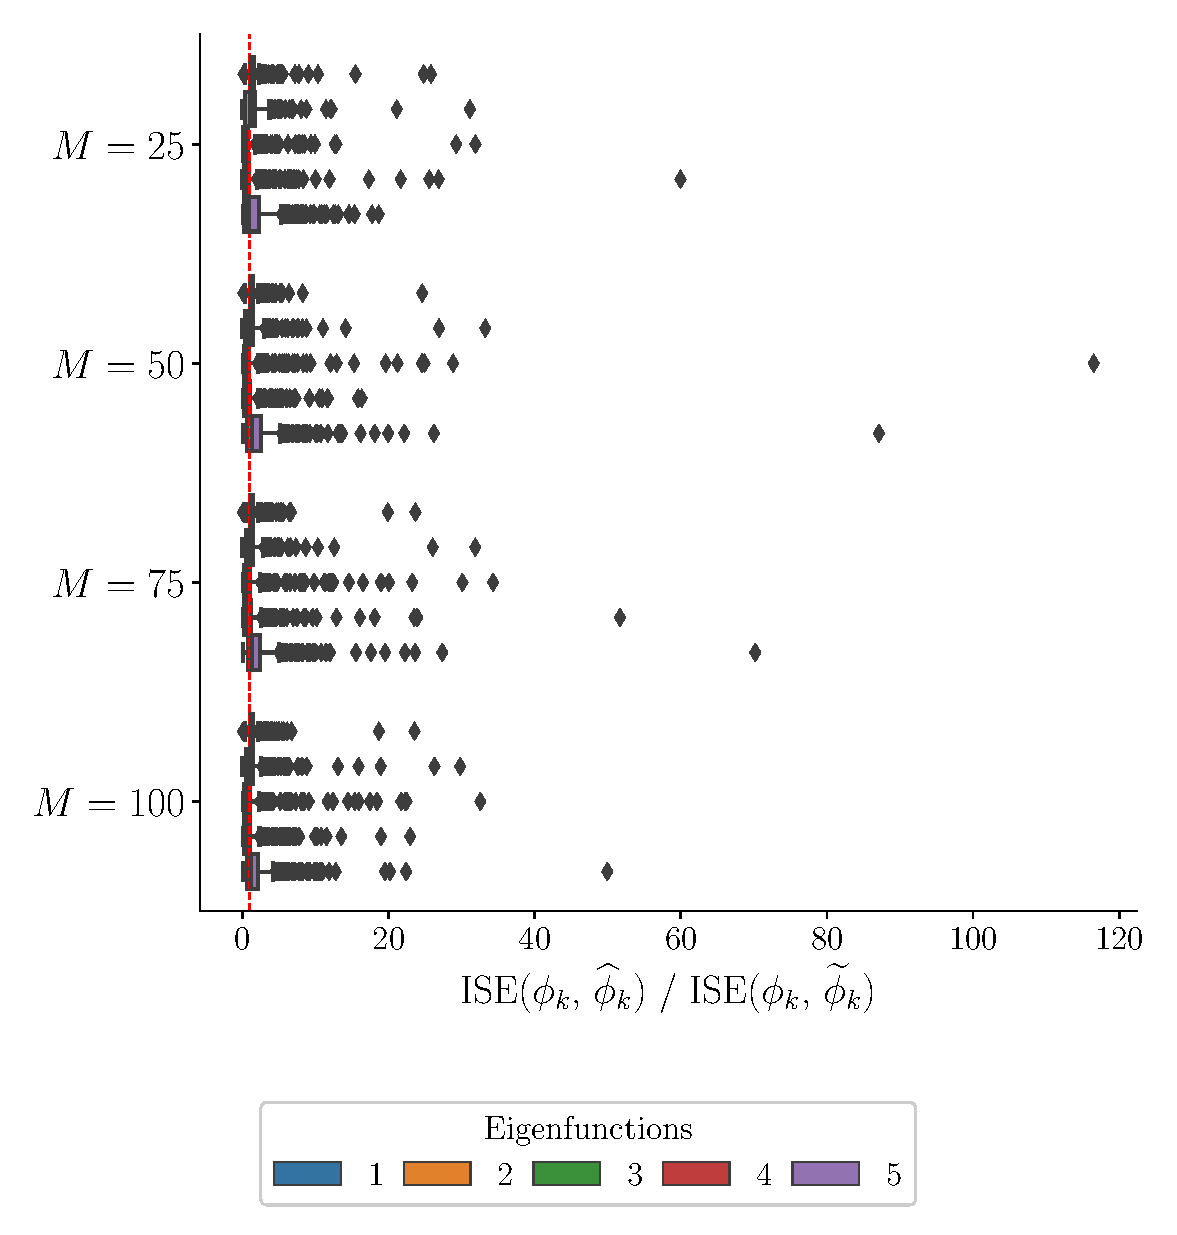
\includegraphics[width=\textwidth]{figures/scenario_2/ise_N25.eps}
         \caption{$N = 25$}
         \label{fig:ise_mfd_2d_25}
     \end{subfigure}
     \hfill
     \begin{subfigure}[b]{0.49\textwidth}
         \centering
         \includegraphics[width=\textwidth]{figures/scenario_2/ise_N50.eps}
         \caption{$N = 50$}
         \label{fig:ise_mfd_2d_50}
     \end{subfigure}
     \\
     \begin{subfigure}[b]{0.49\textwidth}
         \centering
         \includegraphics[width=\textwidth]{figures/scenario_2/ise_N75.eps}
         \caption{$N = 75$}
         \label{fig:ise_mfd_2d_75}
     \end{subfigure}
     \begin{subfigure}[b]{0.49\textwidth}
         \centering
         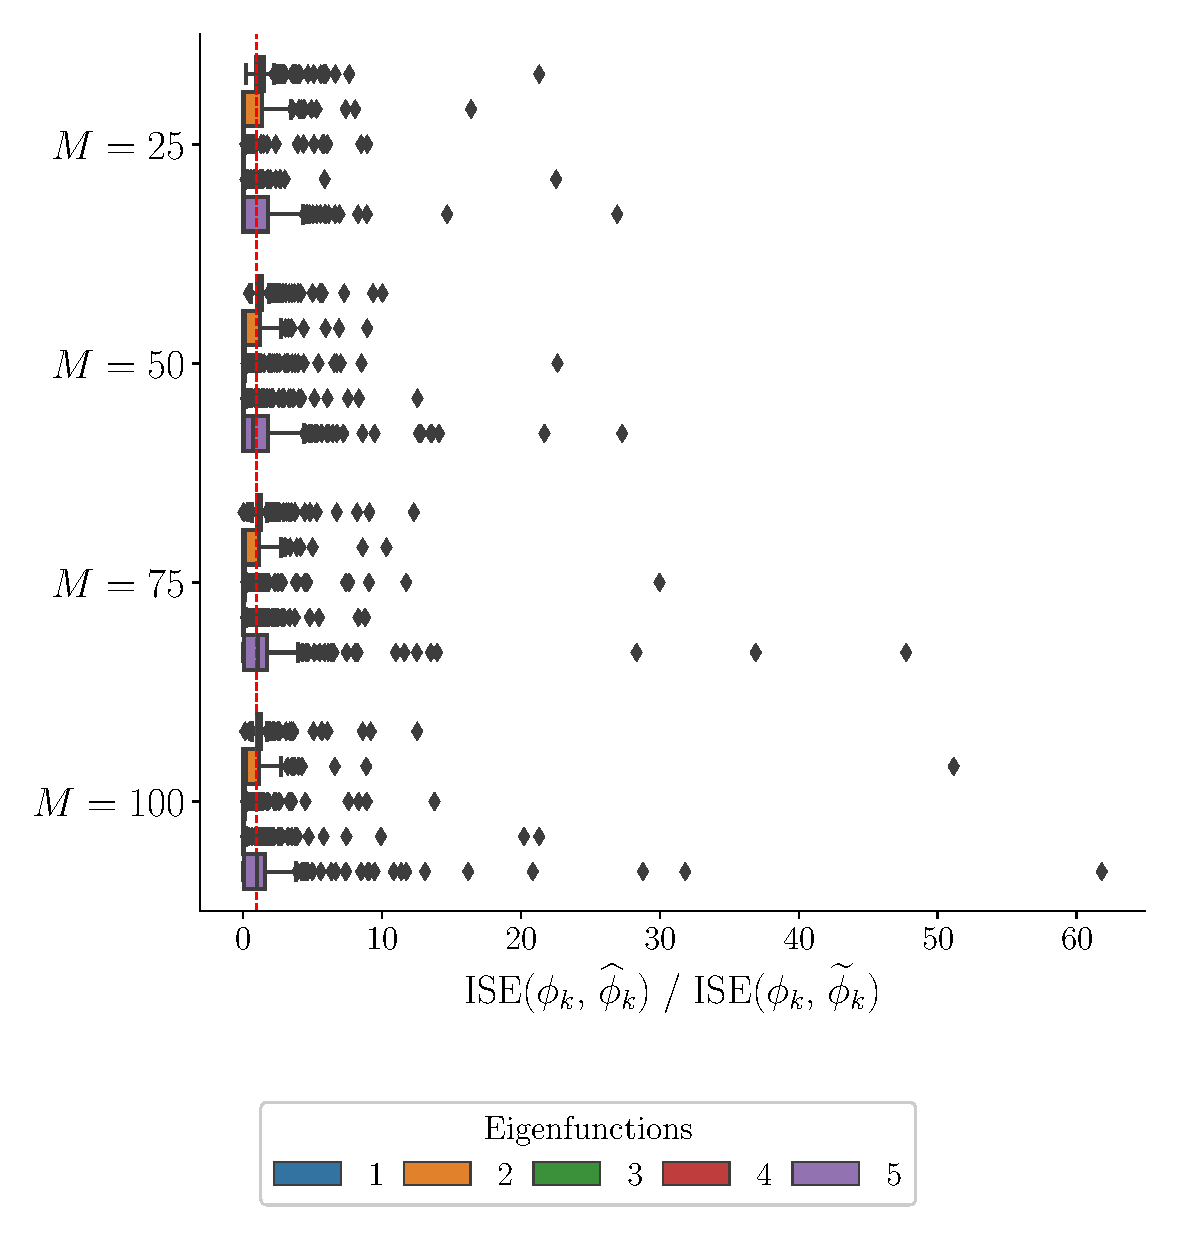
\includegraphics[width=\textwidth]{figures/scenario_2/ise_N100.eps}
         \caption{$N = 100$}
         \label{fig:ise_mfd_2d_100}
    \end{subfigure}
    \caption{ISE for univariate functional data of images data}
    \label{fig:ise_mfd_2d}
\end{figure}

\end{results}

% Curves reconstruction ----------
\begin{results}[Curves reconstruction]

Figure~\ref{fig:mise_mfd_1d} and Figure~\ref{fig:mise_mfd_2d}.

\begin{figure}
     \centering
     \begin{subfigure}[b]{0.49\textwidth}
         \centering
         \includegraphics[width=\textwidth]{figures/scenario_1/mise_N50_M25.eps}
         \caption{$M = 25$}
         \label{fig:mise_mfd_1d_25}
     \end{subfigure}
     \hfill
     \begin{subfigure}[b]{0.49\textwidth}
         \centering
         \includegraphics[width=\textwidth]{figures/scenario_1/mise_N50_M50.eps}
         \caption{$M = 50$}
         \label{fig:mise_mfd_1d_50}
     \end{subfigure}
     \\
     \begin{subfigure}[b]{0.49\textwidth}
         \centering
         \includegraphics[width=\textwidth]{figures/scenario_1/mise_N50_M75.eps}
         \caption{$M = 75$}
         \label{fig:mise_mfd_1d_75}
     \end{subfigure}
     \begin{subfigure}[b]{0.49\textwidth}
         \centering
         \includegraphics[width=\textwidth]{figures/scenario_1/mise_N50_M100.eps}
         \caption{$M = 100$}
         \label{fig:mise_mfd_1d_100}
    \end{subfigure}
    \caption{MISE for multivariate functional data. Each univariate component is defined on a one-dimensional domain. We simulated $N = 50$ observations for each dataset.}
    \label{fig:mise_mfd_1d}
\end{figure}

\begin{figure}
     \centering
     \begin{subfigure}[b]{0.49\textwidth}
         \centering
         \includegraphics[width=\textwidth]{figures/scenario_2/mise_N25.eps}
         \caption{$N = 25$}
         \label{fig:mise_mfd_2d_25}
     \end{subfigure}
     \hfill
     \begin{subfigure}[b]{0.49\textwidth}
         \centering
         \includegraphics[width=\textwidth]{figures/scenario_2/mise_N50.eps}
         \caption{$N = 50$}
         \label{fig:mise_mfd_2d_50}
     \end{subfigure}
     \\
     \begin{subfigure}[b]{0.49\textwidth}
         \centering
         \includegraphics[width=\textwidth]{figures/scenario_2/mise_N75.eps}
         \caption{$N = 75$}
         \label{fig:mise_mfd_2d_75}
     \end{subfigure}
     \begin{subfigure}[b]{0.49\textwidth}
         \centering
         \includegraphics[width=\textwidth]{figures/scenario_2/mise_N100.eps}
         \caption{$N = 100$}
         \label{fig:mise_mfd_2d_100}
    \end{subfigure}
    \caption{MISE for univariate functional data of images data}
    \label{fig:mise_mfd_2d}
\end{figure}

\end{results}


% subsection simulation_results (end)

\subsection{Percentage of variance explained} % (fold)
\label{sub:percentage_of_variance_explained_simulation}

\textcolor{red}{We argue that the percentage of variance explained in \cite{happMultivariateFunctionalPrincipal2018a} is not the good one as they consider the variance explained by each of the components separately and not as a all. Using the inner product matrix however gives the right number of eigenfunctions for a given amount of variance explained.
We also consider the estimation of the number of components to retain to reach a prespecify percentage of variance explained by the data based on the Scenario~1 with $P = 2$, $K = 20$ and we use linear and exponential decreasing of the eigenvalues. The true percentage of variance explained by the $k$th component is given by $\lambda_k / \sum_{k^\prime = 1}^{20} \lambda_{k^\prime}$ and the true percentage of variance explained by the first $K (\leq 20)$ components is given by $\sum_{k = 1}^K \lambda_k / \sum_{k^\prime = 1}^{20} \lambda_{k^\prime}$.
Let fix a certain percentage of variance explained $\alpha \in [0, 1]$. We define $\widetilde{K}$ as the minimum number of components to estimate to reach $100\alpha\%$ of the variance explained,
\begin{equation}
    \widetilde{K} = \arg\min_K \frac{\sum_{k = 1}^K \lambda_k}{\sum_{k^\prime = 1}^{20} \lambda_{k^\prime}} \geq \alpha.
\end{equation}
Using the covariance operator, the implementation of \cite{happMultivariateFunctionalPrincipal2018a} does not allow to directly estimated $\widetilde{K}$ from the multivariate functional data. They propose however to estimate the number of univariate eigenfunctions $K_1$ and $K_2$ based on the percentage of variance explained $\alpha$ for both elements. The number of multivariate eigenfunctions is then set to be $\min\{K_1 + K_2, K\}$ where $K$ is a given scalar. In the simulation, we first run FPCA on each univariate components to estimate the number of components needed to explain $\alpha\%$ of the variance for each components. Then, we run an MFPCA with $K = K_1 + K_2$. Using the Gram matrix, we directly estimated the number of components needed to explain a certain percentage of the variance from the multivariate functional data.
It seems to show that choosing a univariate cut-off within each dimension (e.g., $95\%$), tends to overestimate the final amount of variance – the sum of the final eigenvalues is larger than the sum of the true eigenvalues.}


% subsection percentage_of_variance_explained (end)

% section empirical_analysis (end)

%!TEX root=../main.tex
\section{Application} % (fold)
\label{sec:application}

\textcolor{red}{We apply our methodology utilizing data from the National Basketball Association (NBA). To access comprehensive game data, we utilize the Python package \texttt{nba\_api}\footnote{\url{https://github.com/swar/nba_api/}}, which provides access to the APIs of \url{nba.com}. The dataset encompasses shot location data from all NBA games spanning the seasons between $2018-2019$ and $2022-2023$. Filtering the dataset, we focus solely on players who have made more than $1000$ shots during this five-season period, resulting in a cohort of $131$ players. These players accounted for a total of $493723$ shots attempted, of which $234941$ ($47\%$) were successful. Subsequently, we exclude shots deemed impossible (e.g., out-of-bounds), leaving us with a dataset comprising $492621$ shots (see Figure \ref{fig:shoots_make_miss} for the shots chart of Stephen Curry). To analyze shooting behavior, we employ 2-dimensional kernel density estimation for both the attempted and made shots, utilizing Silverman's rule \citep{silvermanDensityEstimationStatistics1986} for bandwidth estimation. The density estimation is conducted on a regularly spaced grid consisting of $51 \times 51$ points (see Figure \ref{fig:shoots_make_miss} for the estimated densities for Stephen Curry).}

\begin{figure}
    \centering
    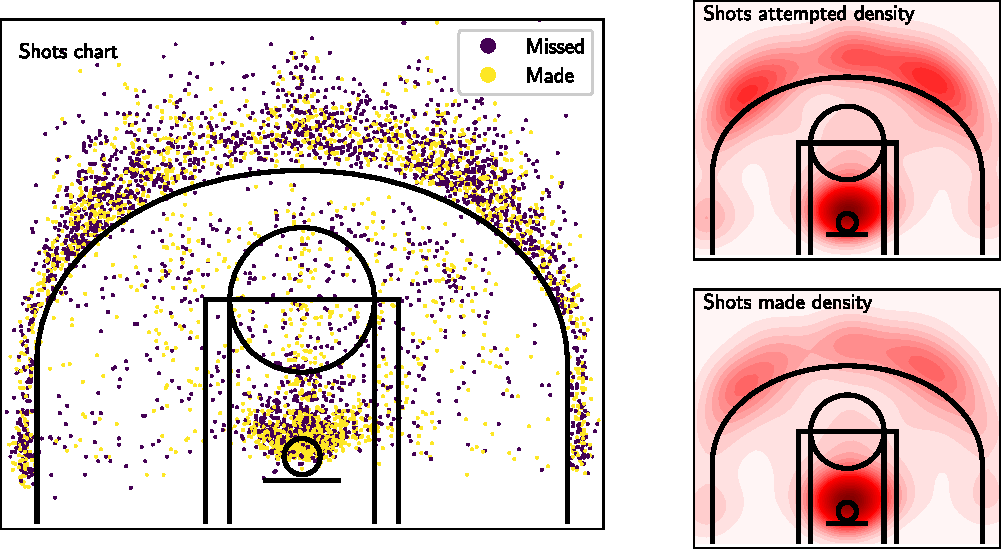
\includegraphics[width=\textwidth]{figures/curry.pdf}
    \caption{\textcolor{red}{Make/Miss shots chart (left) and the estimated densities (right) for Stephen Curry.}}
    \label{fig:shoots_make_miss}
\end{figure}


\textcolor{red}{We estimate the principal components using the decomposition of the Gram matrix and the eigenanalysis of the covariance operator using the FCP-TPA for the univariate components.
%Figure \ref{fig:curry_shoots_decomposition} shows examples of the shooting densities of Stephen Curry and their first five functional principal components using both methods (Figure \ref{fig:curry_decomposition} for the Gram matrix decomposition and Figure \ref{fig:curry_decomposition_fcptpa} for the MFPCA with FCP-TPA.
Remark that the functional principal components, as a representation of the deviation from the mean surface function, may take negative values, while density can only take positive values. For presentation purpose, the functional principal components have been normalized between $-1$ and $1$. Blue corresponds to negative values of the functional components, and thus contribute negatively to the density, while Red corresponds to positive values of the functional components, and thus contribute positively to the density. The bluer the area in the image of the functional components, the smaller/negative the scores, whereas the redder areas correspond to positive values of the scores. The white areas correspond to scores that are closed to $0$, and basically have not impact on the shooting density. The obtained functional components can be explained as different shooting styles.}
\begin{figure}
    \centering
    \begin{subfigure}[b]{0.45\textwidth}
        \centering
        \includegraphics[width=\textwidth]{figures/curry_density.pdf}
        \caption{Curry density}
        \label{fig:curry_density}
    \end{subfigure}
    \\
    \begin{subfigure}[b]{0.45\textwidth}
        \centering
        \includegraphics[width=\textwidth]{figures/curry_gram.pdf}
        \caption{Curry Gram}
        \label{fig:curry_gram}
    \end{subfigure}
    \\
    \begin{subfigure}[b]{0.45\textwidth}
        \centering
        \includegraphics[width=\textwidth]{figures/curry_covariance.pdf}
        \caption{Curry covariance}
        \label{fig:curry_covariance}
    \end{subfigure}
    \caption{Reconstruction.}
    \label{fig:reconstruction}
\end{figure}
\textcolor{red}{For the Gram matrix, the first two principal components and the fourth are related to the shoots under the basket, excluding the other areas. This account for around $95\%$ of the variance. The third and fifth components are related to the three-pointers. These results exhibits the shooting patterns of Stephen Curry. He mostly scores under the basket or behind the three-points line, but almost never in-between. The decomposition of the density of made shots is similar to the ones of attempted shots. We may advance an explanation for that: Stephen Curry does not have a ``weak'' spot, that is somewhere on the court where he shots a lot but does not score.}
% section application (end)

%!TEX root=../main.tex
\section{Discussion and conclusion} % (fold)
\label{sec:discussion}

MFPCA is an interesting tool for analyzing functional data that allows to capture the variability of observations defined by several curves as it extracts the most important modes of variables that explain the covariance structure of the data. We have described the duality between rows and columns of a data matrix in the context of multivariate functional data. We have proposed to use this duality to estimate the eigencomponents of the covariance operator of curves datasets. Comparing the results of the two methods, we propose guidelines to the researcher on which methods to use in which situation. As a summary, if the number of sampling points is a lot larger than the number of observations or if the data in hand are multidimensional (e.g. surfaces), it is preferable to estimate the eigencomponents using the Gram matrix, while if the data are unidimensional with a large number of observations, it is preferable to directly decompose the covariance operator.

\textcolor{red}{Paragraph of the percentage of variance explained.}

\textcolor{red}{In practice, functional data are usually observed with noise. Smoothing each curve individually should be enough to estimate the Gram matrix in this case. Estimating the Gram matrix in the case of sparsely sampled functional data is not relevant as we showed that the Gram matrix is useful when the data is very dense.}

The open-source implementation can be accessed at \url{https://github.com/StevenGolovkine/FDApy}, while scripts to reproduce the simulation are at \url{https://github.com/FAST-ULxNUIG/geom_mfpca}.


% section discussion (end)

% -------------


% APPENDIX ------
\appendix

%!TEX root=../main.tex
\section{Derivation of the inertia of the clouds} % (fold)
\label{sec:derivation_of_the_inertia_of_the_clouds}

In this Section, we derive the inertia of the cloud $\CN$. Recall that 
\begin{equation}\label{eq:var_appendix}
    \Var\{\Xp{p}(t_p)\} = \sum_{n = 1}^N \pi_n \{\Xnp(t_p)\}^2 - \{\mup{p}(t_p)\}^2 \quad\text{where}\quad \mup{p}(t_p) = \sum_{n = 1}^N \pi_n\Xnp(t_p), \quad t_p \in \TT{p}.
\end{equation}

\begin{align*}
    \sum_{n = 1}^N \pi_n d^2(X_n, \mu) &= \sum_{n = 1}^N \pi_n \sum_{p = 1}^P\normLp{\Xnp - \mu^{(p)}}^2\\
    &= \sum_{p = 1}^P\left(\sum_{n = 1}^N \pi_n \normLp{\Xnp}^2 - \normLp{\mup{p}}^2\right) \\
    &= \sum_{p = 1}^P \int_{\TT{p}}\Var{\Xp{p}(t_p)} \dd t_p \\
\sum_{i = 1}^N \sum_{j = 1}^N \pi_i \pi_j d^2(X_i, X_j) &= \sum_{i = 1}^N \sum_{j = 1}^N \pi_i \pi_j \sum_{p = 1}^P \normLp{\Xp{p}_i - \Xp{p}_j}^2\\
    &= \sum_{p = 1}^P \left(2\sum_{i = 1}^N \pi_i\normLp{\Xp{p}_i}^2 - 2\sum_{i = 1}^N \sum_{j = 1}^N \inLp{\Xp{p}_i}{\Xp{p}_j}\right) \\
    &= \sum_{p = 1}^P \left(2\sum_{i = 1}^N \pi_i\normLp{\Xp{p}_i}^2 - 2\normLp{\mup{p}}^2 - 2\sum_{i = 1}^N \sum_{j = 1}^N \inLp{\Xp{p}_i}{\Xp{p}_j} + 2\normLp{\mup{p}}^2\right) \\
    &= 2\sum_{p = 1}^P \int_{\TT{p}}\Var{\Xp{p}(t_p)} \dd t_p
\end{align*}


% section derivation_of_the_inertia_of_the_clouds (end)

%!TEX root=../main.tex
\section{Derivation of the eigencomponents} % (fold)
\label{sec:derivation_of_the_eigencomponents}

Using the Hilbert-Schmidt theorem, there exists a complete orthonormal basis of eigenvectors $\{v_k\}_{1 \leq k \leq N}$ of the inner-product matrix $\mathbf{M}$ such that
\begin{equation}\label{eq:eigen_inner_prod_p}
    \mathbf{M}v_k = l_kv_k.
\end{equation}
Let $X = \left(X_1 - \mu, \dots, X_N - \mu\right)^\top$ and denote $\widetilde{X} = \text{diag}\{\sqrt{\pi_1}, \dots, \sqrt{\pi_N}\}X$, the matrix of weighted observations. Recall that, in the case of $P$-dimensional process, the realisations of the process $X_n,~n = 1, \cdots, N$ and $\mu$ are vectors of functions of length $P$, and thus $X$ (and $\widetilde{X}$) is a matrix of functions of size $N \times P$. By left multiplying Equation~\eqref{eq:eigen_inner_prod_p} by $\widetilde{X}^\top$, we obtain
\begin{equation}\label{eq:eigen_inner_prod_left}
    \widetilde{X}^\top \mathbf{M} v_k = l_k \widetilde{X}^\top v_k.
\end{equation} 
Expanding Equation~\eqref{eq:eigen_inner_prod_left}, for each component $p = 1, \dots, P$, we have,
\begin{equation}\label{eq:inner_prod_p}
    \sum_{i = 1}^N \sum_{j = 1}^N \pi_i \sqrt{\pi_j}[v_{k}]_j\left\{X_i^{(p)}(\cdot) - \mu^{(p)}(\cdot)\right\}\inH{X_i - \mu}{X_j - \mu} = l_k \mkern-5mu\sum_{n = 1}^N \mkern-4mu\sqrt{\pi_n}[v_{k}]_n\left\{\Xnp(\cdot) - \mu^{(p)}(\cdot)\right\}.
\end{equation}
Here and in the following, we note $[a]_p$ the $p$th entry of the vector $a$. Starting from the left side of Equation~\eqref{eq:inner_prod_p}, we get
\begin{align}\label{eq:inner_prod_p_left}
[\widetilde{X}^\top \mathbf{M} v_k]_p &= \sum_{i = 1}^N \sum_{j = 1}^N \pi_i \sqrt{\pi_j} [v_{k}]_j \left\{X_i^{(p)}(\cdot) - \mu^{(p)}(\cdot)\right\}\inH{X_i - \mu}{X_j - \mu}\\
&= \sum_{q = 1}^P \int_{\TT{q}} \sum_{i = 1}^N \pi_i\left\{X_i^{(p)}(\cdot) - \mu^{(p)}(\cdot)\right\} \left\{X_i^{(q)}(s_q) - \mu^{(q)}(s_q)\right\}  \\
&\quad\quad \sum_{j = 1}^N \sqrt{\pi_j}[v_{k}]_j \left\{X_j^{(q)}(s_q) - \mu^{(q)}(s_q)\right\} \dd s_q \\
&= \sum_{q = 1}^P \int_{\TT{q}} C_{pq}(\cdot, s_q)\sum_{j = 1}^N \sqrt{\pi_j}[v_{k}]_j \left\{X_j^{(q)}(s_q) - \mu^{(q)}(s_q)\right\} \dd s_q \\
&= \sum_{j = 1}^N \inH{C_{p \cdot}(\cdot, \cdot)}{\sqrt{\pi_j}[v_{k}]_j \left\{X_j - \mu\right\}} \\
&= \Gamma\left(\sum_{j = 1}^N \sqrt{\pi_j}[v_{k}]_j \left\{X_j - \mu\right\} \right)^{\mkern-9mu(p)}\mkern-18mu(\cdot)
\end{align}
and, starting from the right side of Equation~\eqref{eq:inner_prod_p},
\begin{equation}\label{eq:inner_prod_p_right}
    [l_k \widetilde{X}^\top v_k]_p = l_k \sum_{n = 1}^N \sqrt{\pi_n}[v_{k}]_n \left\{\Xnp(\cdot) - \mu^{(p)}(\cdot)\right\}.
\end{equation}
From Equation~\eqref{eq:inner_prod_p_left} and Equation~\eqref{eq:inner_prod_p_right}, we obtain
\begin{equation}
    \Gamma\left(\sum_{j = 1}^N \sqrt{\pi_j}[v_{k}]_j \left\{X_j - \mu\right\}\right)^{\mkern-9mu(p)}\mkern-18mu(\cdot) = l_k \sum_{n = 1}^N \sqrt{\pi_n}[v_{k}]_n \left\{\Xnp(\cdot) - \mu^{(p)}(\cdot)\right\}, \quad\text{for all}~ p = 1, \dots, P.
\end{equation}
By identification in Equation~\eqref{eq:eigendecomposition}, we find that, for each components $p$,
\begin{equation}\label{eq:eigen_estimation}
\lambda_k = l_k \quad\text{and}\quad \phi_k^{(p)}(\cdot) = \sum_{n = 1}^N \sqrt{\pi_n}[v_{k}]_n \left\{\Xnp(\cdot) - \mu^{(p)}(\cdot)\right\}, \quad k \geq 1.
\end{equation}
For $k \geq 1$, the norm of the eigenfunction is computed as the following:
\begin{align*}
\normH{\phi_k}^2 &= \sum_{i = 1}^N \sum_{j = 1}^N \sqrt{\pi_i\pi_j}[v_{k}]_i [v_{k}]_j\inH{X_i - \mu}{X_j - \mu} = \sum_{i = 1}^N [v_{k}]_i \sum_{j = 1}^N \mathbf{M}_{ij} [v_{k}]_j \\
    &= \sum_{i = 1}^N [v_{k}]_i l_k [v_{k}]_i = l_k \normLp{v_k}^2 = l_k. \\
\end{align*}
Therefore, in order to have an orthonormal basis of eigenfunctions, we normalise the eigenfunctions $\phi_k$ from Equation~\eqref{eq:eigen_estimation} by $1 / \sqrt{l_k}$.
Concerning the estimation of the scores, for $n = 1, \dots, N$, for $k \geq 1$, we have
\begin{align}
    \mathfrak{c}_{nk} &= \inH{X_n - \mu}{\phi_k} = \frac{1}{\sqrt{l_k}}\sum_{j = 1}^N \sqrt{\pi_j}[v_{k}]_j \inH{X_n - \mu}{X_j - \mu}\\
    &= \frac{1}{\sqrt{l_k\pi_n}}\sum_{j = 1}^N [v_{k}]_j \mathbf{M}_{nj} = \sqrt{\frac{l_k}{\pi_n}}[v_{k}]_n.\\
\end{align}

Concerning the expansion of the data into the basis of function $\Psi$, we write 
\begin{equation}
    M = \left(\text{diag}\{
        \sqrt{\pi_1}, \dots, \sqrt{\pi_N}\}\left(\mathrm{I}_{\!N} - \mathbf{1}_{\!N}\Pi^\top\right) \mathbf{C}W^{1/2}\right)\left(\text{diag}\{
        \sqrt{\pi_1}, \dots, \sqrt{\pi_N}\}\left(\mathrm{I}_{\!N} - \mathbf{1}_{\!N}\Pi^\top\right) \mathbf{C}W^{1/2}\right)^\top.
\end{equation}
We note
\begin{equation}
    \mathbf{A} = \text{diag}\{\sqrt{\pi_1}, \dots, \sqrt{\pi_N}\}\left(\mathrm{I}_{\!N} - \mathbf{1}_{\!N}\Pi^\top\right) \mathbf{C}W^{1/2},
\end{equation}
such that $\mathbf{M} = \mathbf{A}\mathbf{A}^\top$.
We also assume that $\phi_1, \phi_2, \dots$ the eigenfunctions of the covariance operator $\Gamma$ have a decomposition into the basis $\Psi$
\begin{equation}
    \phi_k(\cdot) = 
        \begin{pmatrix} 
            \phi_k^{(1)}(\cdot) \\
            \vdots \\
            \phi_k^{(P)}(\cdot)
        \end{pmatrix} = 
        \begin{pmatrix} 
            \psi^{(1) \top}(\cdot) b_{1k} \\
            \vdots \\
            \psi^{(P) \top}(\cdot) b_{Pk}
        \end{pmatrix}, \quad\text{where}\quad
        b_{pk} = \left(b_{p k 1}, \dots, b_{p k K_p} \right)^\top.
\end{equation}

We have, for $p = 1, \dots, P$,
\begin{align*}
    \left(\Gamma \phi_k\right)^{(p)}(\cdot) &= \sum_{q = 1}^P \int_{\TT{q}} C_{p q}(\cdot, s_q)\phi_k^{(q)}(s_q) \dd s_q \\
    &= \sum_{q = 1}^P \int_{\TT{q}} \Psi(\cdot)^{(p) \top} \mathbf{C}^{(p) \top} \left(\text{diag}\{\pi_1, \dots, \pi_N\} - \Pi\Pi^\top\right)\mathbf{C}^{(q)} \Psi^{(q)}(s_q) \Psi^{(q)}(s_q)^\top b_{q k} \dd s_q \\
    &= \Psi(\cdot)^{(p) \top} \mathbf{C}^{(p) \top} \left(\text{diag}\{\pi_1, \dots, \pi_N\} - \Pi\Pi^\top\right)\sum_{q = 1}^P \mathbf{C}^{(q)} \int_{\TT{q}} \Psi^{(q)}(s_q) \Psi(s_q)^{(q) \top} \dd s_q b_{q k} \\
    &= \Psi(\cdot)^{(p) \top} \mathbf{C}^{(p) \top} \left(\text{diag}\{\pi_1, \dots, \pi_N\} - \Pi\Pi^\top\right) \sum_{q = 1}^P \mathbf{C}^{(q)} \mathbf{W}^{(q)} b_{q k}. \\
\end{align*}
This equation is true for all $p = 1, \cdots, P$, this can be rewritten with matrices as
\begin{equation}
    \Gamma \phi_k(\cdot) = \Psi(\cdot)^{\top} \mathbf{C}^{\top} \left(\text{diag}\{\pi_1, \dots, \pi_N\} - \Pi\Pi^\top\right) \mathbf{C} \mathbf{W} b_{k}.
\end{equation}
From the eigenequation, we have that
\begin{equation}
    \Gamma \phi_k(\cdot) = \lambda_k \phi_k(\cdot) \Longleftrightarrow \Psi(\cdot)^{\top} \mathbf{C}^{\top} \left(\text{diag}\{\pi_1, \dots, \pi_N\} - \Pi\Pi^\top\right) \mathbf{C} \mathbf{W} b_{k} = \lambda_k \Psi(\cdot)^\top b_k.
\end{equation}
Since this equation must be true for all $t_p \in \TT{p}$, this imply the equation
\begin{equation}\label{eq:eigen_decom}
    \mathbf{C}^{\top} \left(\text{diag}\{\pi_1, \dots, \pi_N\} - \Pi\Pi^\top\right) \mathbf{C} \mathbf{W} b_{k} = \lambda_k b_k.
\end{equation}
As the eigenfunctions are assumed to be normalized, $\normH{\phi_k}^2 = 1$. And so, $b_k^\top W b_k = 1$. Let $u_k = W^{1/2}b_k$. Then, from Equation \eqref{eq:eigen_decom}, we obtain
\begin{equation}\label{eq:eigen_cov_op}
    \mathbf{W}^{1/2} \mathbf{C}^{\top} \left(\text{diag}\{\pi_1, \dots, \pi_N\} - \Pi\Pi^\top\right) \mathbf{C} \mathbf{W}^{1/2} u_k = \lambda_k u_k \Longleftrightarrow \mathbf{A}^\top\mathbf{A} u_k = N\lambda_k u_k.
\end{equation}
From the eigendecomposition of the matrix $M$, we get
\begin{equation}\label{eq:eigen_inner_prod}
    \mathbf{M}v_k = l_k v_k \Longleftrightarrow \mathbf{A}\mathbf{A}^\top v_k = l_k v_k.
\end{equation}
The equations \eqref{eq:eigen_cov_op} and \eqref{eq:eigen_inner_prod} are eigenequations in the classical PCA case, with the duality $X^\top X$ and $XX^\top$. Following \cite{pagesMultipleFactorAnalysis2014,hardleAppliedMultivariateStatistical2019}, we find that, for $1 \leq k \leq K$,
\begin{equation}
    \lambda_k = l_k, \quad v_k = \frac{1}{\sqrt{l_k}}\mathbf{A} u_k \quad\text{and}\quad u_k = \frac{1}{\sqrt{l_k}} \mathbf{A}^\top v_k.
\end{equation}
And finally, to get the coefficient of the eigenfunctions, for $1 \leq k \leq K$,
\begin{equation}
    b_k = \mathbf{W}^{-1/2}u_k = \frac{1}{\sqrt{l_k}} \mathbf{C}^\top \left(\mathrm{I}_{\!N} - \Pi\mathbf{1}_{\!N}^\top\right) \text{diag}\{\sqrt{\pi_1}, \dots, \sqrt{\pi_N}\}v_k.
\end{equation}

% section derivation_of_the_eigencomponents (end)

%!TEX root=../main.tex
\section{More results} % (fold)
\label{sec:more_results}


\subsection{Simulation} % (fold)
\label{sub:simulation}

\textcolor{red}{We present the results of the simulations in the sparse and noisy cases. Figures \ref{fig:logAE_mfd_1d_noise}, \ref{fig:ise_mfd_1d_noise} and \ref{fig:mise_mfd_1d_noise} present the boxplots of the RSE, ISE and MRSE, respectively, for the noisy case. To generate noisy data, we consider the model \eqref{eq:model_error} where $\sigma^2 = 0.25$. For the \texttt{(Tensor) PCA} method, we first smooth the 2-dimensional data using P-Splines smoothing and estimate a smooth version of the mean and covariance functions for the one-dimensional data using P-Splines smoothing. For the \texttt{2D/1D B-Splines} and \texttt{Gram} methods, all the observations have been smoothed using P-Splines smoothing beforehand. In every case, the penalty involved in P-Splines smoothing has been estimated using cross-validation.}

\begin{figure}
    \centering
    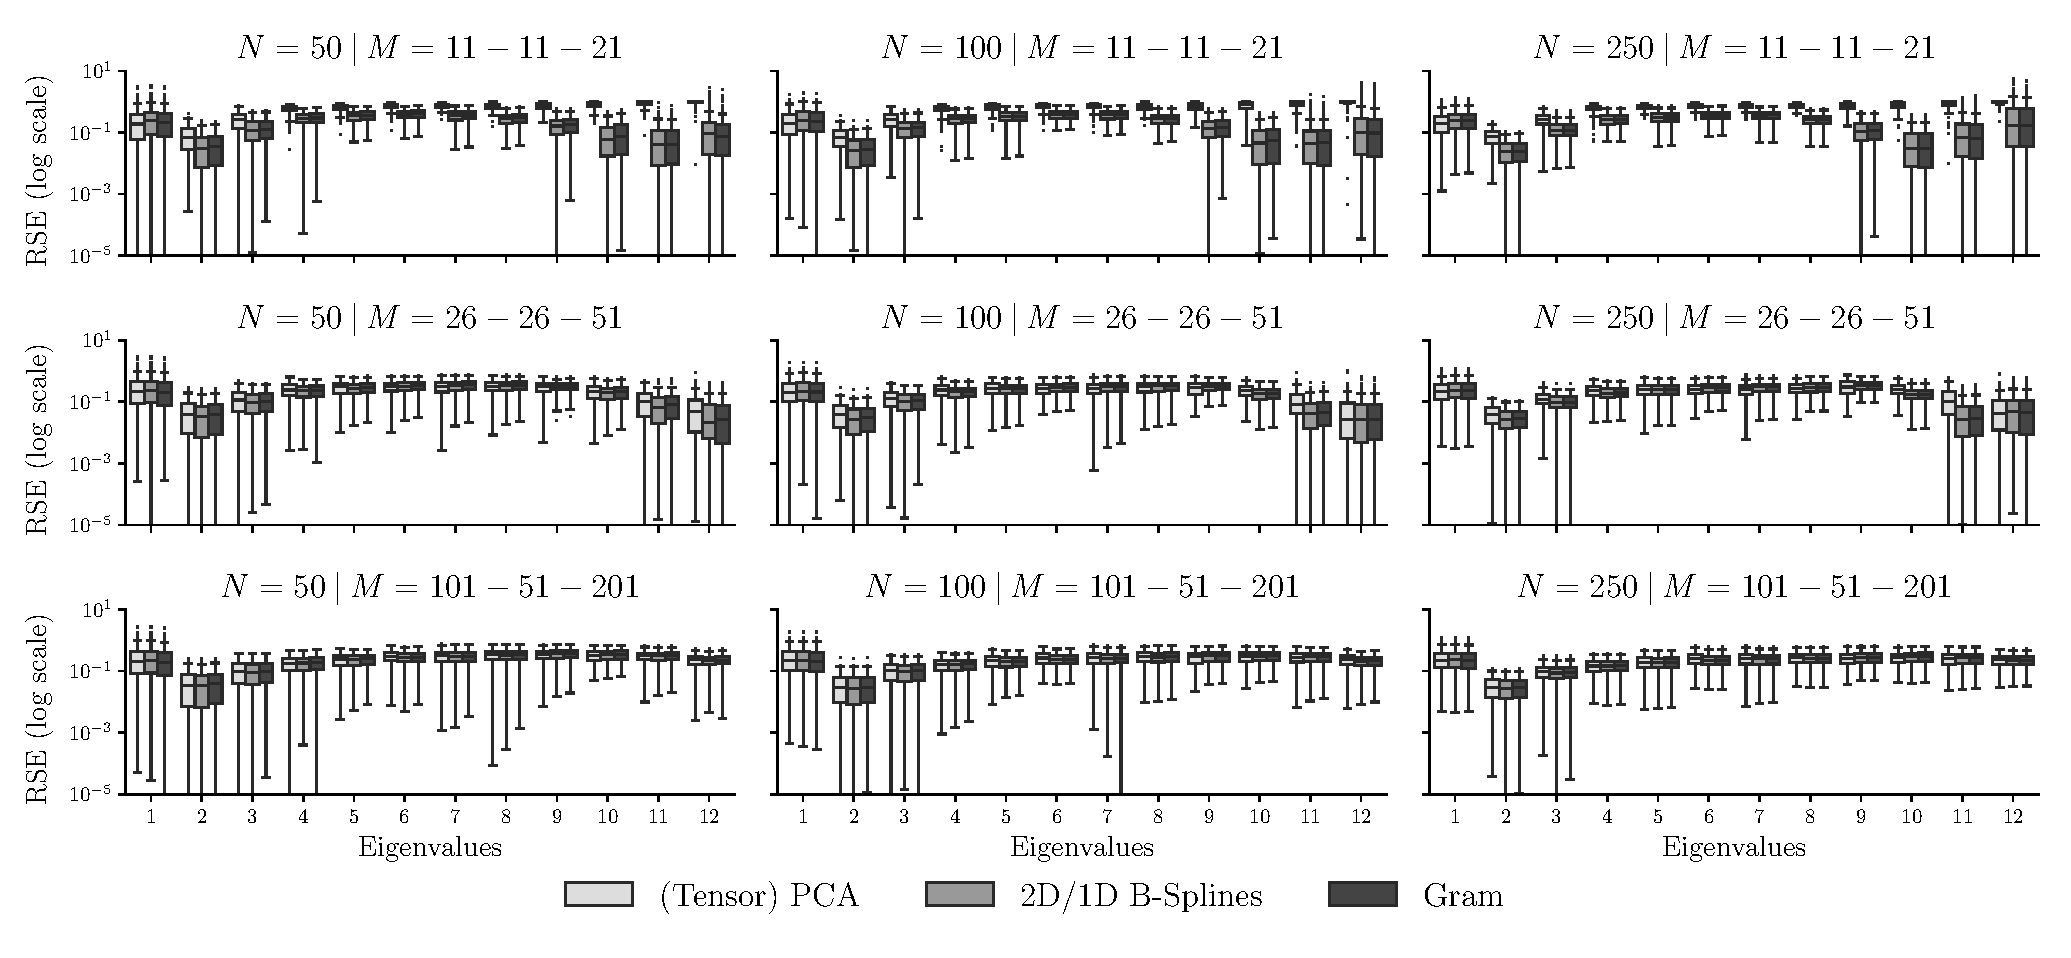
\includegraphics[width=0.95\textwidth]{figures/AE_noise.eps}
    \caption{\textcolor{red}{RSE for the estimated eigenvalues for each method in the noisy case. $N$ is the number of observations, $M$ is the number of sampling points per curve (the first two numbers are for the images and the last one is for the curves).}}
    \label{fig:logAE_mfd_1d_noise}
\end{figure}

\begin{figure}
    \centering
    \includegraphics[width=0.8\textwidth]{figures/AE_sparse.eps}
    \caption{\textcolor{red}{RSE for the estimated eigenvalues for each method in the sparse case. We set $N = 250$, $M^{(1)} = 101 \times 51$ and $M^{(2)} = 201$. For the case of medium sparsity, we remove $50\%-70\%$ of the sampling points and for the case of high sparsity, we remove $90\%-95\%$ of the sampling points.}}
    \label{fig:logAE_mfd_1d_sparse}
\end{figure}


\textcolor{red}{Figures \ref{fig:logAE_mfd_1d_sparse}, \ref{fig:ise_mfd_1d_sparse} and \ref{fig:mise_mfd_1d_sparse} present the boxplots of the RSE, ISE and MRSE, respectively, for the sparse. In this case, we only consider $N = 250$, $M^{(1)} = 101 \times 51$, $M^{(2)} = 201$ and no noise. We consider medium sparsity, where $50\%-70\%$ of the sampling points have been removed and high sparsity, where $90\%-95\%$ of the sampling points have been removed. For the \texttt{(Tensor) PCA} method, we first interpolate the 2-dimensional data to have the observations reguarlarly sampled on a grid and estimate a smooth version of the mean and covariance functions for the one-dimensional data using P-Splines smoothing. For the \texttt{2D/1D B-Splines} method, all the observations have been smoothed using P-splines smoothing with a penalty estimated by cross-validation. For the \texttt{Gram} method, the observations have been linearly interpolated to estimate the inner-product matrix.}



\begin{figure}
     \centering
    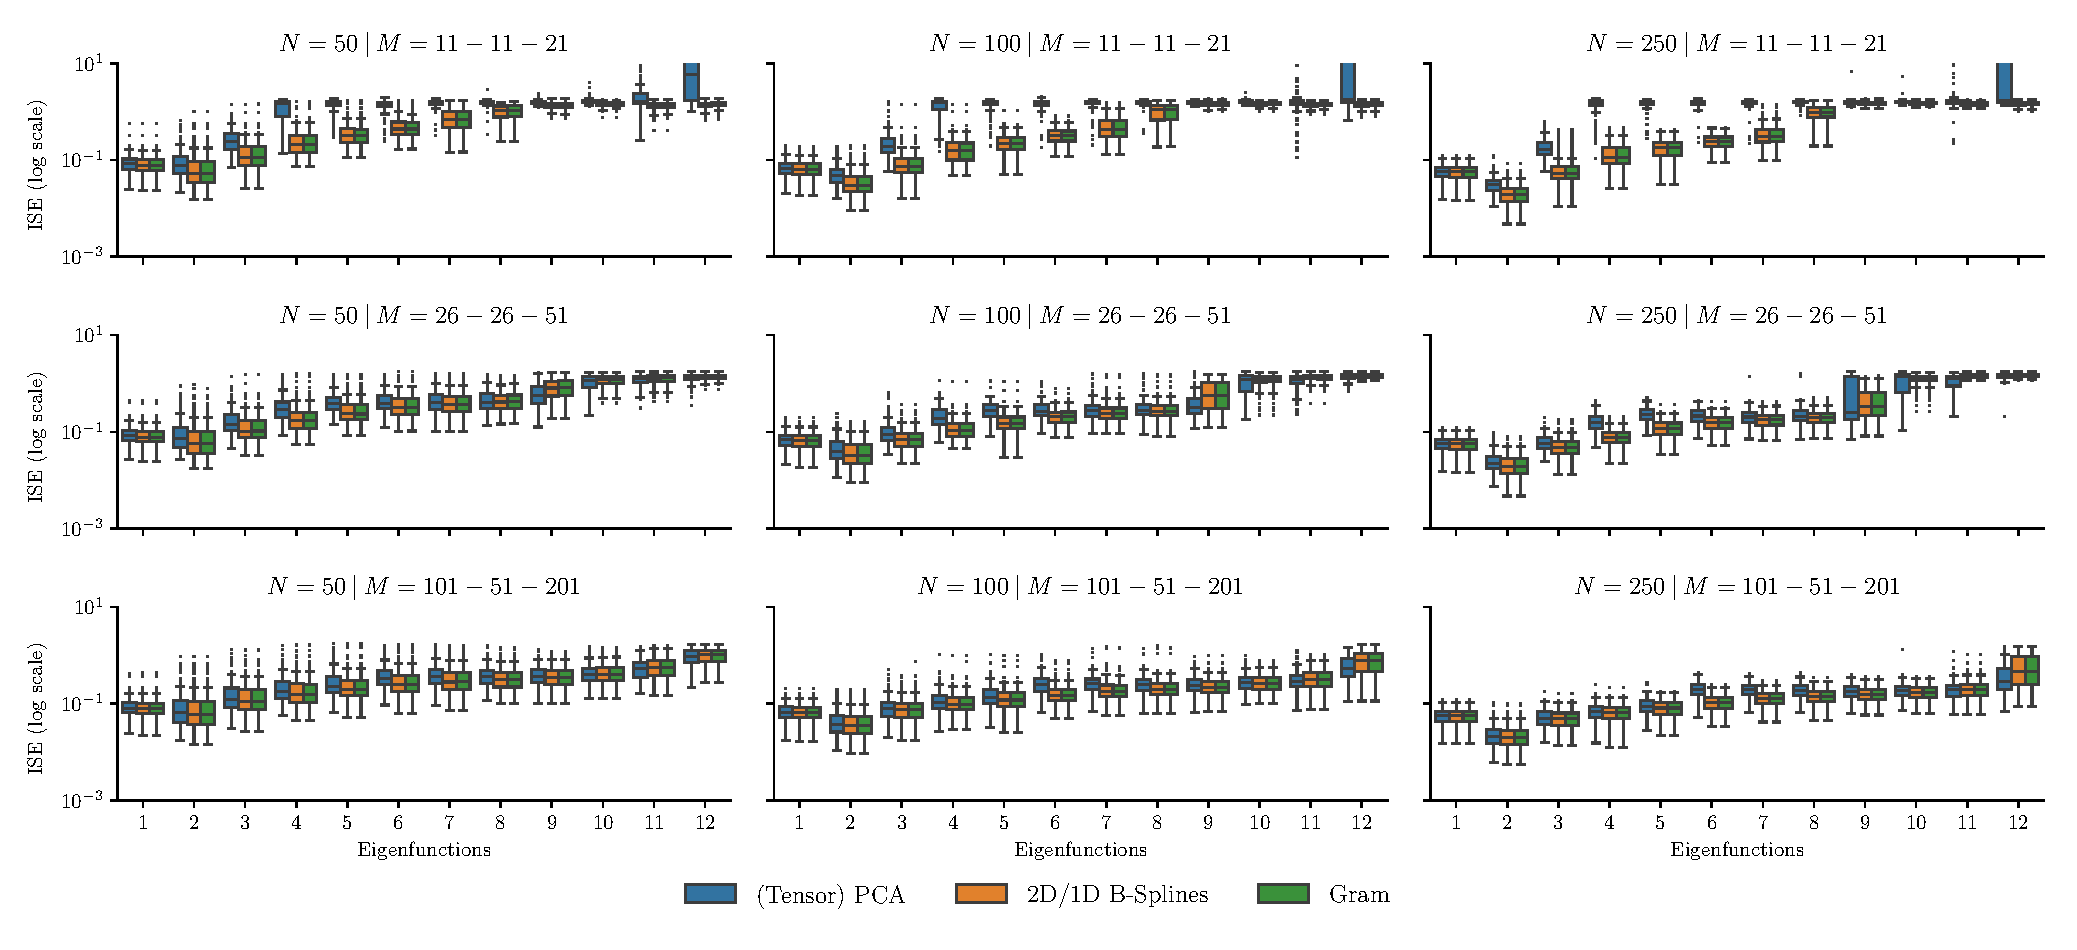
\includegraphics[width=0.95\textwidth]{figures/ISE_noise.eps}
    \caption{\textcolor{red}{ISE for the estimated eigenfunctions for each method in the noisy case. $N$ is the number of observations, $M$ is the number of sampling points per curve (the first two numbers are for the images and the last one is for the curves).}}
    \label{fig:ise_mfd_1d_noise}
\end{figure}

\begin{figure}
     \centering
    \includegraphics[width=0.95\textwidth]{figures/ISE_sparse.eps}
    \caption{\textcolor{red}{ISE for the estimated eigenfunctions for each method in the sparse case. We set $N = 250$, $M^{(1)} = 101 \times 51$ and $M^{(2)} = 201$. For the case of medium sparsity, we remove $50\%-70\%$ of the sampling points and for the case of high sparsity, we remove $90\%-95\%$ of the sampling points.}}
    \label{fig:ise_mfd_1d_sparse}
\end{figure}


\begin{figure}
     \centering
     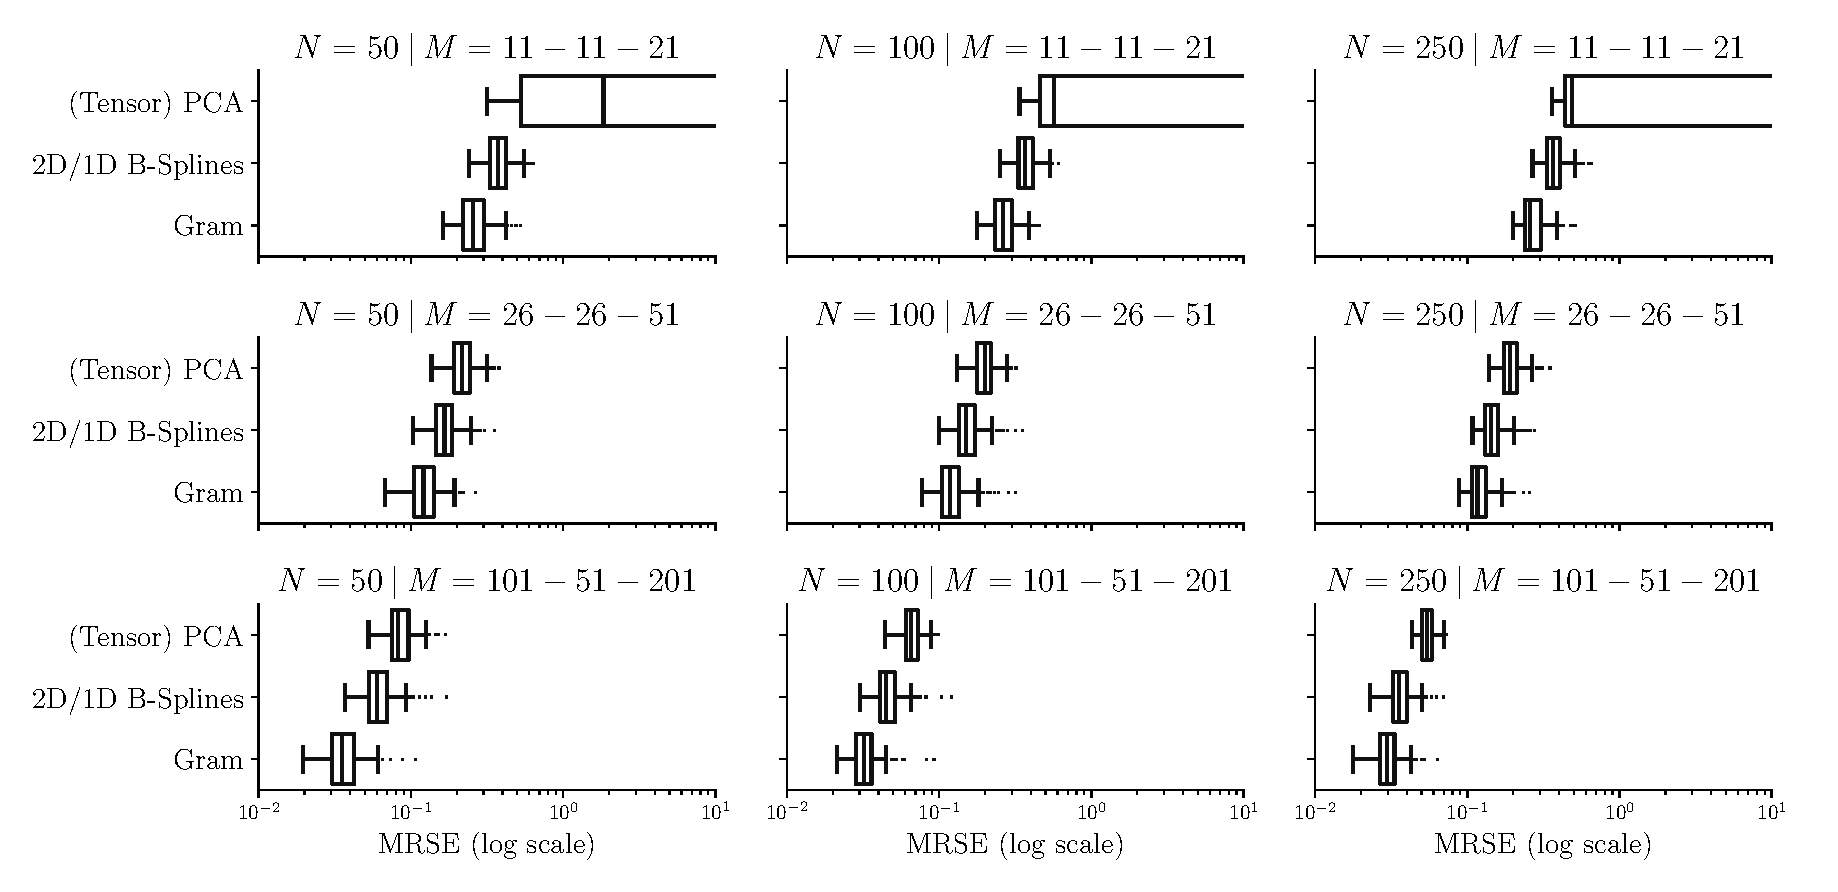
\includegraphics[width=0.95\textwidth]{figures/MRSE_noise.eps}
    \caption{\textcolor{red}{MRSE for the reconstructed curves for each method in the noisy case. $N$ is the number of observations, $M$ is the number of sampling points per curve (the first two numbers are for the images and the last one is for the curves).}}
    \label{fig:mise_mfd_1d_noise}
\end{figure}

\begin{figure}
     \centering
     \includegraphics[width=0.95\textwidth]{figures/MRSE_sparse.eps}
    \caption{\textcolor{red}{MRSE for the reconstructed curves for each method in the sparse case. We set $N = 250$, $M^{(1)} = 101 \times 51$ and $M^{(2)} = 201$. For the case of medium sparsity, we remove $50\%-70\%$ of the sampling points and for the case of high sparsity, we remove $90\%-95\%$ of the sampling points.}}
    \label{fig:mise_mfd_1d_sparse}
\end{figure}

% subsection simulation (end)

\subsection{Application} % (fold)
\label{sub:application}

% \begin{figure}
%     \centering
%     \begin{subfigure}[b]{0.45\textwidth}
%         \centering
%         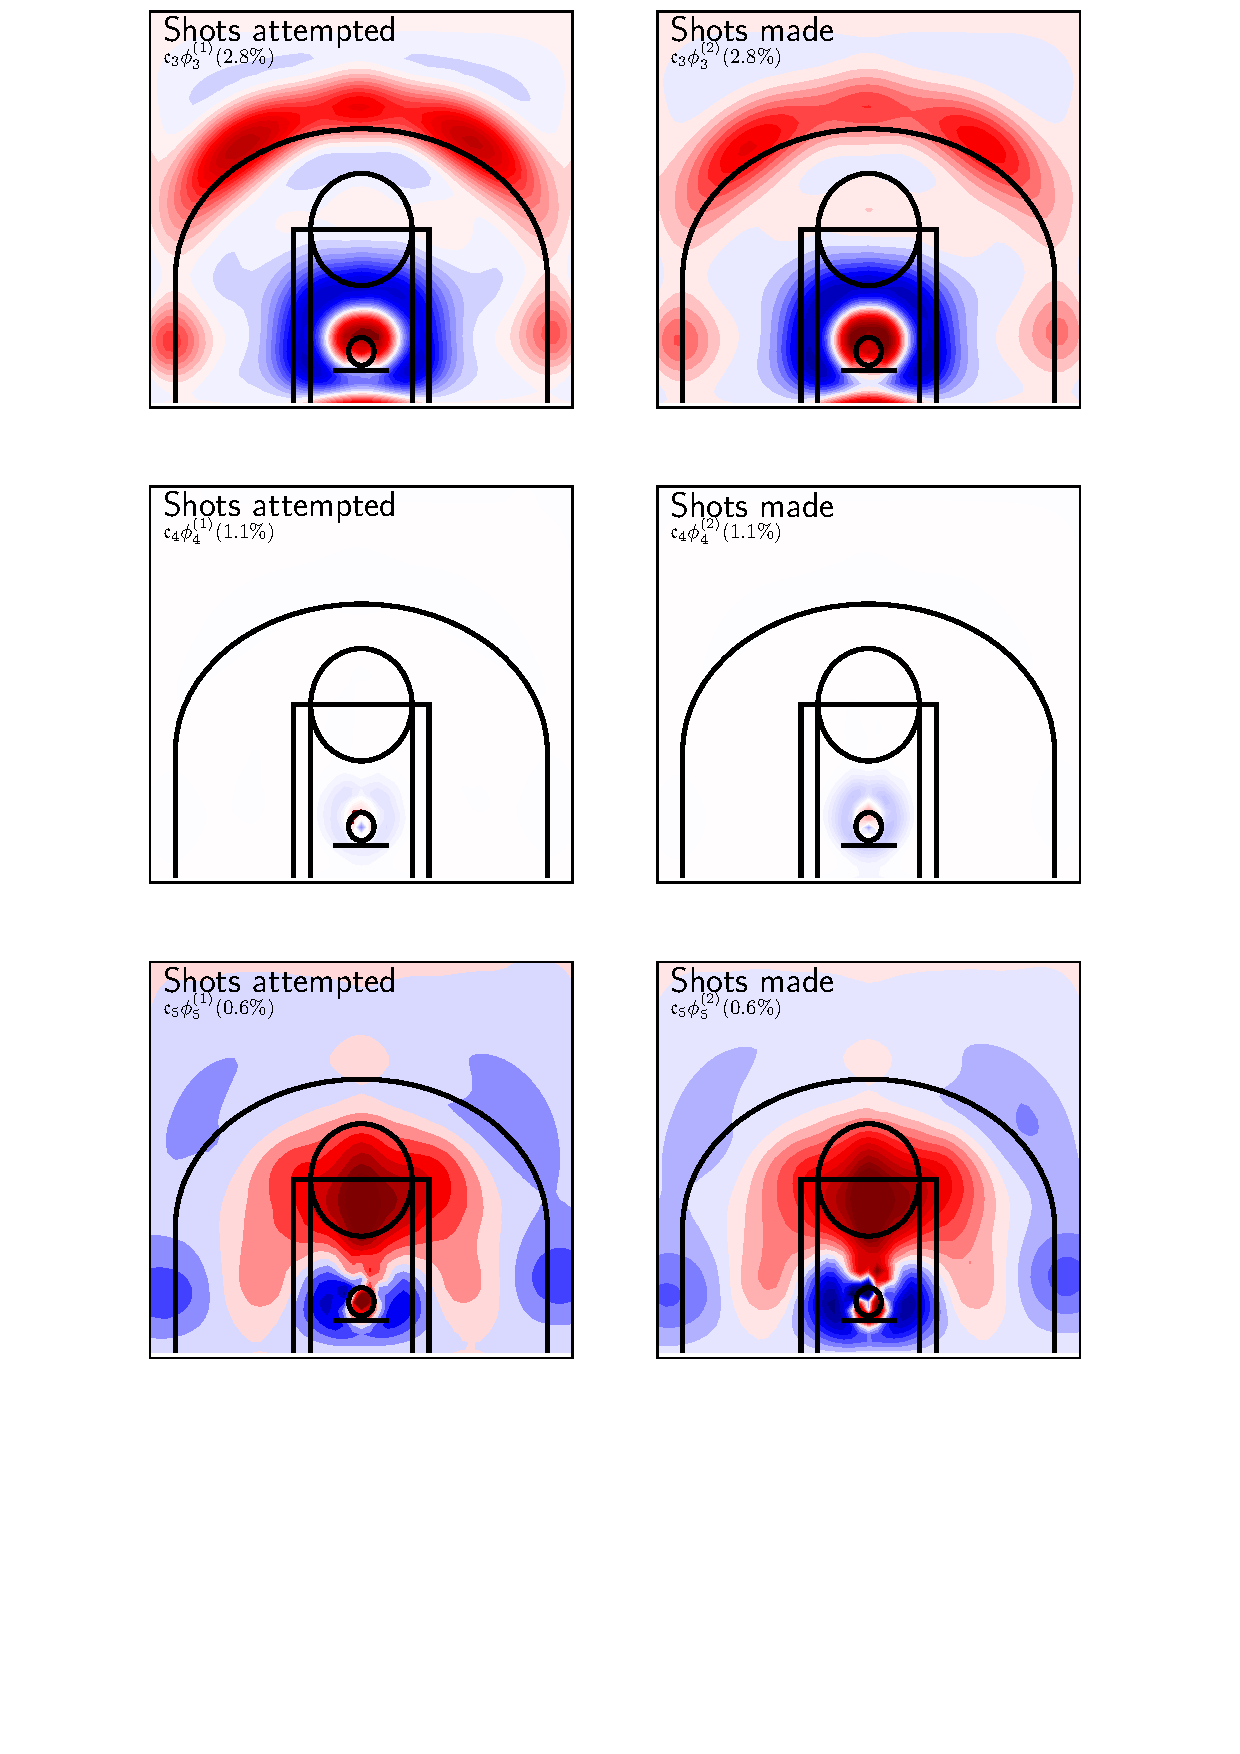
\includegraphics[width=\textwidth]{figures/durant_decomposition.pdf}
%         \caption{Gram matrix}
%         \label{fig:durant_decomposition}
%     \end{subfigure}
%     \hfill
%     \begin{subfigure}[b]{0.45\textwidth}
%         \centering
%         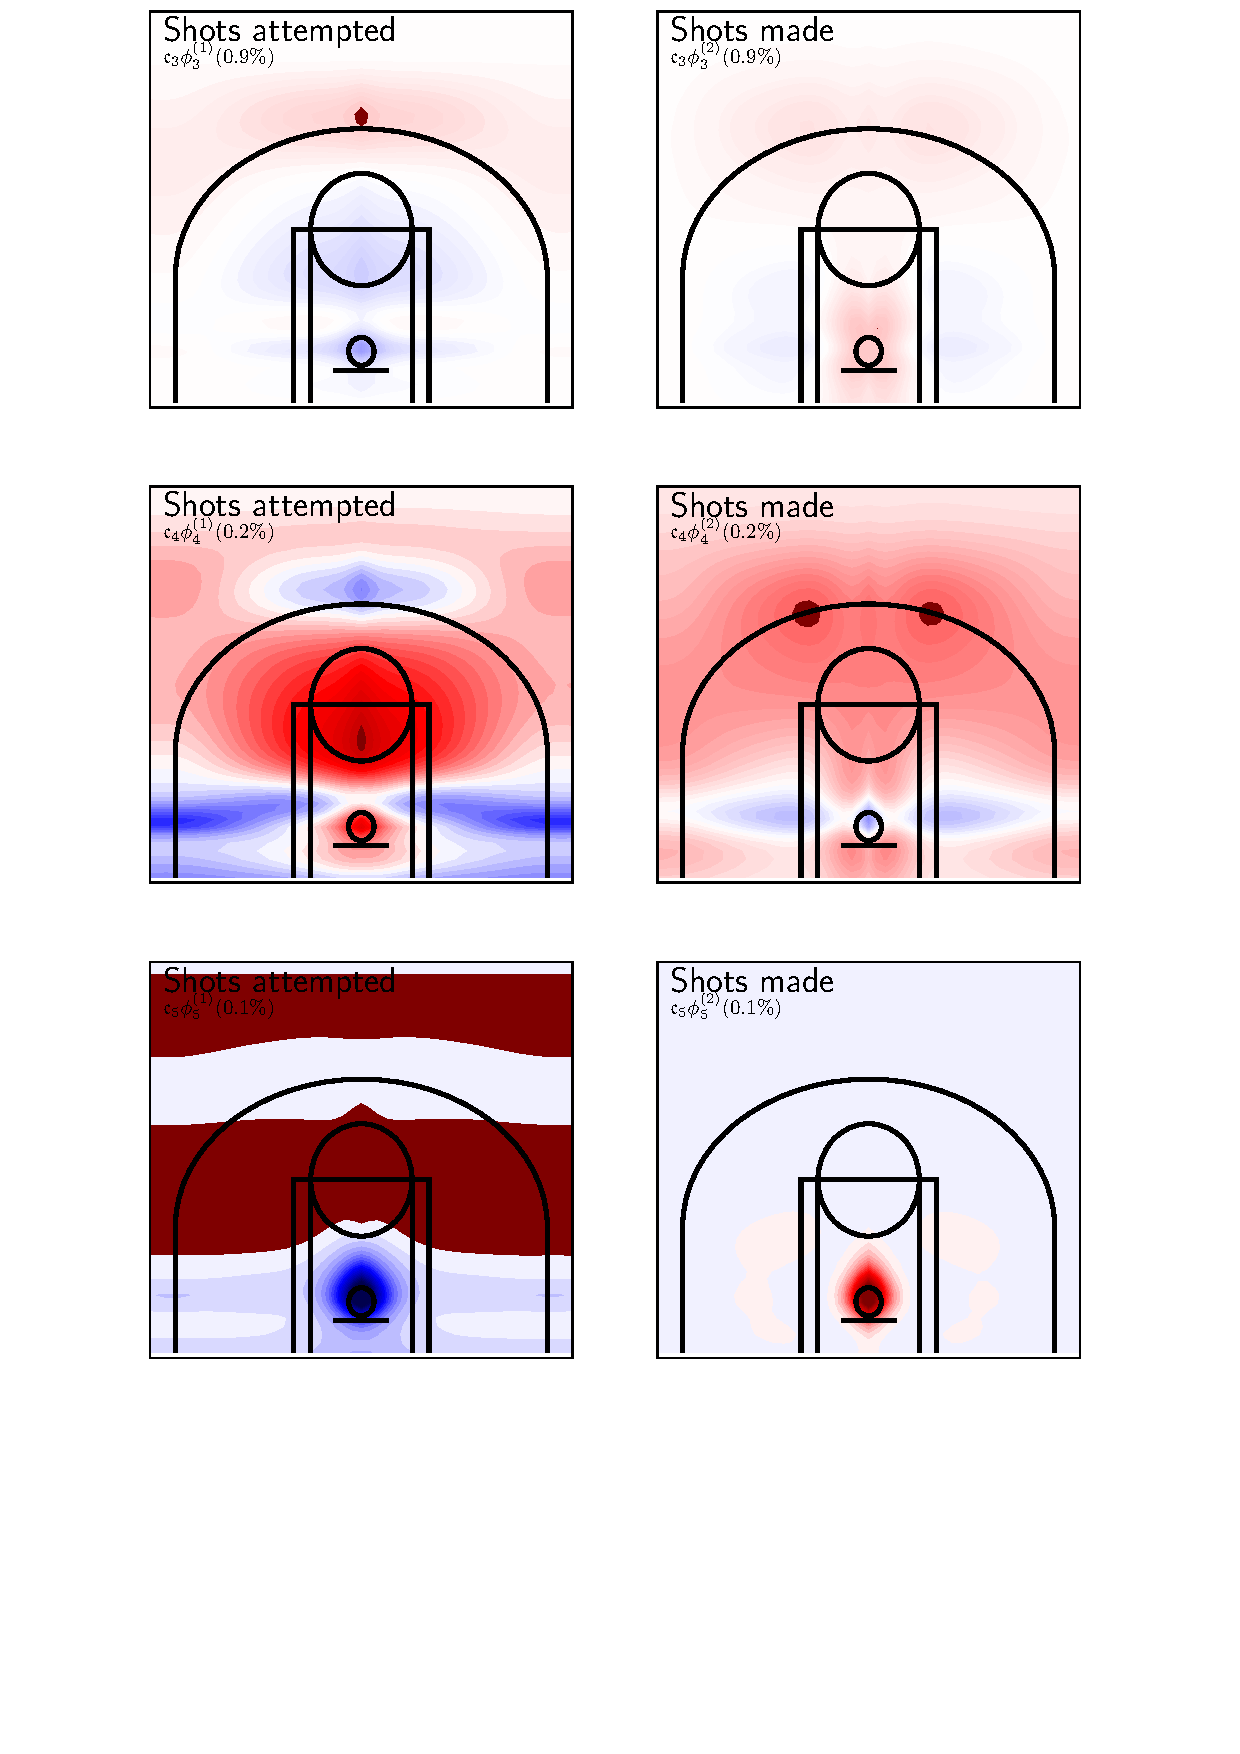
\includegraphics[width=\textwidth]{figures/durant_decomposition_fcptpa.pdf}
%         \caption{FCPTPA}
%         \label{fig:durant_decomposition_fcptpa}
%     \end{subfigure}
%     \caption{Decomposition for Kevin Durant.}
%     \label{fig:durant_shoots_decomposition}
% \end{figure}

% subsection application (end)

% section more_results (end)


% ACKNOWLEDGMENT -------
\section*{Acknowledgment}

S. Golovkine, A. J. Simpkin and N. Bargary are partially supported by Science Foundation Ireland under Grant No. 19/FFP/7002 and co-funded under the European Regional Development Fund. E. Gunning is supported in part Science Foundation Ireland (Grant No. 18/CRT/6049) and co-funded under the European Regional Development Fund.

% REFERENCES ---------
\bibliographystyle{apalike}
\bibliography{./biblio.bib}

\end{document}

